% -*- coding: utf-8 -*-

\begin{chapter}{Экваториальные процессы}\label{chap:14}
% \chapter{Equatorial Processes}
Изучение процессов, протекающих в океане в районе экватора, важно для
оценки влияния океана на атмосферу, поскольку именно они определяют межгодовые 
флуктуации в глобальной климатической системе. Солнце%
\index{Солнце!нагрев экваториальных вод} обогревает обширные
пространства Тихого и Индийского океанов в тропических широтах, в
результате чего происходит интенсивное испарение морской
воды. Впоследствии, при формировании осадков, высвобождается значительное
количество тепла, в результате чего эти районы являются первичным
источником атмосферной циркуляции\index{атмосферная циркуляция!причины} 
(рис.~\ref{fig:rainheat}). Количество осадков%
\index{количество осадков!экваториальных},
выпадающих над этими обширными территориями, превышает~$3\mpyr$
(рис.~\ref{fig:precip}), а в некоторых районах достигает даже~$5\mpyr$. 
Чтобы лучше пояснить значение этих величин в общей картине, отметим,
что при количестве осадков~$5\mpyr$
в атмосферу высвобождается в среднем $400\wpsqm$ тепла. Экваториальные
течения изменяют интенсивность процессов обмена на границе океан-атмосфера, 
в особенности посредством такого явления, как Эль-Ниньо, последствия которого
глобальны. В настоящей главе
приводится описание основных экваториальных процессов, их многолетней
изменчивости и её влияния на климат.
%
% Equatorial processes are at the center of our understanding the
% influence of the ocean on the atmosphere, and they dominate the
% interannual fluctuations in global weather patterns. The
% sun\index{sun!warms equatorial watewrs} warms the vast expanses of the
% tropical Pacific and Indian ocean, evaporating water. When the water
% condenses as rain it releases so much heat that these areas are the
% primary engine driving the atmospheric circulation\index{atmospheric
% circulation!causes} (figure 14.1). Rainfall\index{rainfall!equatorial}
% over extensive areas exceeds three meters per year (figure 5.5), and
% some oceanic regions receive more than five meters of rain per
% year. To put the numbers in perspective, five meters of rain per year
% releases on average 400 W/m$^2$ of heat to the atmosphere. Equatorial
% currents modulate the air-sea interactions, especially through the
% phenomenon known as El Ni\~{n}o, with global consequences. I describe
% here first the basic equatorial processes, then the year-to-year
% variability of the processes and the influence of the variability on
% weather patterns.

\begin{figure}[b!]
\vspace{-3ex}
\makebox[120mm] [c]{\includegraphics{pics/rainheat}}
\caption{Средний диабатический нагрев атмосферы на интервале~$700$--$50\mBar$
в декабре, январе и феврале, вычисленный по данным~ECMWF за 1983--1989~гг.
Преобладающим источником тепла служит выделение скрытого тепла при
образовании осадков. (Webster, et al. 1992).}
\label{fig:rainheat}
\end{figure}
%
% \begin{figure}[b!]
% \vspace{-3ex}
% \makebox[120mm] [c]{\includegraphics{rainheat}}
% \footnotesize
% Figure 14.1 Average diabatic \rule{0pt}{3ex}heating between 700 and 50
% mb in the atmosphere during December, January and February calculated
% from \textsc{ecmwf} data for 1983--1989. Most of the heating is due to
% the release of latent heat by rain.  After Webster et al. (1992).
% \label{fig:rainheat}
% %\vspace{-4ex}
% \end{figure}

\begin{section}{Экваториальные процессы}
% \section{Equatorial Processes}
\index{экваториальные процессы}%
Тропические регионы характеризуются тонким постоянным неглубоким
слоем теплых вод, находящихся над глубинными холодными слоями. В этом
аспекте вертикальная стратификация водной толщи в тропиках схожа со
стратификацией в высоких широтах в летний период. Поверхностная температура 
воды наиболее высока на западе (рис.~\ref{fig:SSTvariability}) 
in the great Pacific-warm pool. 
Глубина перемешанного слоя\index{перемешанный слой!экваториальный} 
велика на западе и очень мала на востоке (рис.~\ref{fig:equator}).
%
% \index{equatorial processes}The tropical ocean is characterized by a
% thin, permanent, shallow layer of warm water over deeper, colder
% water. In this respect, the vertical stratification is similar to the
% summer stratification at higher latitudes. Surface waters are hottest
% in the west (figure 6.3) in the great Pacific warm pool. The mixed
% layer\index{mixed layer!equatorial} is deep in the west and very
% shallow in the east (Figure 14.2).

\begin{figure}[t!]
\begin{centering}
\makebox[120mm] [c]{\includegraphics{pics/equator}}
\end{centering}
\caption{Средняя температура верхнего слоя Тихого океана вдоль экватора от
северной части Новой Гвинеи до Эквадора, рассчитанная по данным
(Levitus, 1982).}  
\label{fig:equator}
\vspace{-2ex}
\end{figure}
%
% \begin{figure}[t!]
% \centering
% \makebox[120mm] [c]{\includegraphics{equator}}
% \footnotesize
% Figure 14.2 The mean, \rule{0pt}{3ex}upper-ocean, thermal structure
% along the equator in the Pacific from north of New Guinea to Ecuador
% calculated from data in Levitus (1982).
%
% \label{fig:equator}
% \vspace{-2ex}
% \end{figure}

Наличие мелкого термоклина\index{термоклин!мелкий} имеет важные последствия. 
Юго-восточные пассаты дуют вдоль экватора (рис.~\ref{fig:surfacewinds}), 
проявляя тенденцию к усилению на востоке. 
К северу от экватора экмановский перенос\index{экмановский перенос}%
\index{перенос!экваториальный} имеет
северное направление, а к югу от экватора~--- южное. Экмановская дивергенция
приводит к апвеллингу\index{апвеллинг!экваториальный}  на экваторе. На западе
апвеллинговые воды теплые, но на востоке~--- холодные, потому что термоклин
настолько неглубок. Это приводит к появлению холодного языка воды на
поверхности океана, простирающегося от берегов Южной Америки
практически до линии смены дат (рис.~\ref{fig:SSTvariability}). 
%
% The shallow thermocline\index{thermocline!shallow} has important
% consequences. The southeast trade winds blow along the equator (figure
% 4.2) although they tend to be strongest in the east. North of the
% equator, Ekman transport\index{Ekman
% transport}\index{transport!equatorial} is northward. South of the
% equator it is southward. The divergence of the Ekman flow causes
% upwelling\index{upwelling!equatorial} on the equator. In the west, the
% upwelled water is warm. But in the east the upwelled water is cold
% because the thermocline is so shallow.  This leads to a cold tongue of
% water at the sea surface extending from South America to near the
% dateline (figure 6.3).


Температура поверхностного слоя\index{поверхностная температура}%
\index{температура!поверхностная} на востоке является результатом баланса 
четырех составляющих:
%
% Surface temperature\index{surface
% temperature}\index{temperature!surface} in the east is a balance among
% four processes:
\begin{enumparen}

\item
интенсивности апвеллинга\index{апвеллинг!экваториальный}, которая определяется 
западной компонентой ветра;
%% westward -- "с запада" или "на запад"?
%
% \vitem The strength of the upwelling\index{upwelling!equatorial},
% which is determined by the westward component of the wind.

\item
скорости направленных на запад течений, которые переносят холодные воды
от побережья Перу и Эквадора;
%
% \vitem The speed of westward currents which carry cold water from the
% coast of Peru and Ecuador.

\item
перемешивания\index{перемешивание!экваториальное} <<север-юг>> с теплыми 
водами по обеим сторонам от экватора;
%
% \vitem North-south mixing\index{mixing!equatorial} with warmer waters
% on either side of the equator.

\item
потоков тепла через поверхность океана вдоль экватора. 
%
% \vitem Heat fluxes through the sea surface along the equator.
\end{enumparen}

Наличие температурного градиента в направлении с востока на запад
вдоль экватора приводит к появлению зональной циркуляции в
атмосфере~--- циркуляции Уолкера. Грозовые штормы
над теплым бассейном переносят воздух снизу вверх, а на востоке опускающийся
воздух подпитывает обратный поток к поверхности. Изменения
температурного градиента влияют на циркуляцию Уолкера, а она, в свою
очередь, влияет на сам градиент. Эта обратная связь может приводить к
нестабильности, известной под названием Эль-Ниньо-Южная осцилляция (ENSO)%
\index{Южная осцилляция!индекс}%
\index{Южная осцилляция!Эль-Ниньо-Южная осцилляция (ENSO)},
которую мы рассмотрим в следующем разделе.
%
% The east-west temperature gradient on the equator drives a zonal
% circulation in the atmosphere, the Walker circulation. Thunderstorms
% over the warm pool carry air upward, and sinking air in the east feeds
% the return flow at the surface. Variations in the temperature gradient
% influences the Walker circulation, which, in turn, influences the
% gradient. The feedback can lead to an instability, the El
% Ni\~{n}o-Southern Oscillation (\textsc{enso})\index{Southern
% Oscillation!Index}\index{Southern Oscillation!El Ni\~{n}o Southern
% Oscillation (ENSO)} discussed in the next section.

\begin{paragraph}{Поверхностные течения.}
%\paragraph{Surface Currents}
\index{течения!поверхностные}\index{поверхностные течения}
Сильная стратификация ограничивает влияние ветровой циркуляции
перемешанным слоем\index{перемешанный слой!течения} 
и верхним термоклином\index{термокли!верхний}. Теория Свердрупа и её 
дальнейшее развитие~--- теория Манка, изложенные в 
разд.~\ref{sec:SverdrupTheory} и~\ref{sec:MunksSolution}, объясняют
поверхностные течения в тропических частях Атлантического, Тихого и
Индийского океанов. Система течений включает (рис.~\ref{fig:EqCurr}):
%
% \index{currents!surface}\index{surface currents}The strong
% stratification confines the wind-driven circulation to the mixed
% layer\index{mixed layer!currents} and upper
% thermocline\index{thermocline!upper}. Sverdrup's theory and Munk's
% extension, described in \S11.1 and \S11.3, explain the surface
% currents in the tropical Atlantic, Pacific, and Indian ocean. The
% currents include (figure 14.3):

\begin{figure}[t!]
\makebox[120mm] [c]{\includegraphics{pics/EqCurr}}
\caption{Средние направления и скорости течений на глубине~$10\m$,
вычисленные по Модульной модели океана на основе данных о ветрах и осредненных
потоках тепла\index{поток тепла} за период с~1981 по~1994~г. Эта модель,
используемая Национальными центрами по прогнозированию окружающей среды
NOAA, усваивает данные наблюдений поверхностной и подповерхностной 
температуры. (Behringer, Ji, and Leetmaa,1998)}
\label{fig:EqCurr}
\end{figure}
%
% \begin{figure}[t!]
% %\vspace{-1ex}
% \makebox[120mm] [c]{\includegraphics{EqCurr}}
% \footnotesize
% Figure 14.3 Average currents at 10 m \rule{0pt}{3ex}calculated from
% the Modular Ocean Model driven by observed winds and mean heat
% fluxes\index{heat flux} from 1981 to 1994. The model, operated by the
% \textsc{noaa} National Centers for Environmental Prediction,
% assimilates observed surface and subsurface temperatures. After
% Behringer, Ji, and Leetmaa (1998).
% \label{fig:EqCurr}
% \vspace{-4ex}
% \end{figure}

\begin{enumerate}
\item
Северное экваториальное противотечение между~\latlon{3}{N}
и~\latlon{10}{N}, направленное к востоку со средней скоростью поверхностного
потока около $50\cmps$.  Оно находится в центре действия слабых ветров, в так
называемом \emph{поясе штилей}\index{пояс штилей|textbf}, расположенном в
районе~5--\latlon{10}{N}, сходятся северные и южные пассаты 
(другое название этой области~--- \emph{внутритропическая зона конвергенции}%
\index{внутритропическая зона конвергенции|textbf}).
%
% \vitem The North Equatorial Countercurrent between 3\degrees N and
% 10\degrees N, which flows eastward with a typical surface speed of 50
% cm/s. The current is centered on the band of weak winds, the
% \textit{doldrums}\index{doldrums|textbf}, around 5--10\degrees N where
% the north and south trade winds converge, the \textit{tropical
% convergence zone}\index{tropical convergence zone|textbf}.

\item
Северное и Южное экваториальные течения, направленные к
западу. Располагаются по обе стороны от экваториального
противотечения. Эти течения неглубокие, распространяются на глубины,
не превышающие~$200\m$. Северное течение слабое, со скоростью потока
около~$20\cmps$. Скорость же южного течения может достигать~$100\cmps$
в зоне между~\latlon{3}{N} и экватором.
%
% \vitem The North and South Equatorial Currents which flow westward in
% the zonal band on either side of the countercurrent. The currents are
% shallow, less than 200 m deep. The northern current is weak, with a
% speed less than roughly 20 cm/s.  The southern current has a maximum
% speed of around 100 cm/s, in the band between 3\degrees N and the
% equator.
\end{enumerate}

Течения в Атлантическом океане имеют схожий характер с течениями в
Тихом океане, потому что пассаты в Атлантике также сходятся около
5--\latlon{10}{N}. Южное экваториальное течение в Атлантическом океане
следует в северо-западном направлении вдоль побережья Бразилии, где
оно превращается в так называемое Северо-Бразильское течение. В
Индийском океане пояс штилей находится в южном полушарии и существует
только в период зимы северного полушария. В северном полушарии течения
имеют обратное направление под действием муссонов.
%
% The currents in the Atlantic are similar to those in the Pacific
% because the trade winds in that ocean also converge near 5\degrees
% --10\degrees N.  The South Equatorial Current in the Atlantic
% continues northwest along the coast of Brazil, where it is known as
% the North Brazil Current. In the Indian Ocean, the doldrums occur in
% the southern hemisphere and only during the northern-hemisphere
% winter. In the northern hemisphere, the currents reverse with the
% monsoon winds.

Отметим, что это далеко не все, что можно сказать об экваториальных течениях.
%
% There is, however, much more to the story of equatorial currents.
\end{paragraph}

\begin{paragraph}{Экваториальное подповерхностное течение: наблюдения.}
% \paragraph{Equatorial Undercurrent: Observations}
\index{экваториальные процессы!подповерхностное течение}%
В районе экватора на глубине всего лишь нескольких метров существует
сильный поток в восточном направлении~--- Экваториальное
подповерхностное течение, последнее крупное открытие в системе течений 
Мирового океана. История его обнаружения такова:
%
% \index{equatorial processes!undercurrent}Just a few meters below the
% surface on the equator is a strong eastward flowing current, the
% Equatorial Undercurrent, the last major oceanic current to be
% discovered. Here's the story:
\begin{quotation}
В сентябре 1951~г.\ научно-исследовательское судно Службы рыбных ресурсов 
и дикой природы США вело ярусный лов рыбы в районе экватора южнее Гавайских 
островов. В ходе работ было замечено, что погруженные в воду орудия лова 
устойчиво дрейфуют в восточном направлении. В следующем году Кромвелл вместе 
с Монтгомери и Строупом возглавили экспедицию для исследования вертикального 
распределения горизонтальных скоростей движения морской воды на экваторе. 
Используя плавучие якоря, устанавливаемые на поверхности и на различных 
глубинах, они обнаружили в центральном районе Тихого океана сильное узкое
течение в нижней части поверхностного слоя и верхней части термоклина
\index{термоклин!верхняя часть}, 
направленное к востоку (Cromwell, et al., 1954). Несколько лет спустя,
экспедиция \textit{Eastropac} института им.~Скриппса, которой также
руководил Кромвелл, выяснила, что течение простирается на восток вплоть 
до Галапагосских островов, но при этом оно отсутствует
между этими островами и Южно-Американским континентом.
%
% In September 1951, aboard the U.S. Fish and Wildlife Service research
% vessel long-line fishing on the equator south of Hawaii, it was
% noticed that the subsurface gear drifted steadily to the east. The
% next year Cromwell, in company with Montgomery and Stroup, led an
% expedition to investigate the vertical distribution of horizontal
% velocity at the equator. Using floating drogues at the surface and at
% various depths, they were able to establish the presence, near the
% equator in the central Pacific, of a strong, narrow eastward current
% in the lower part of the surface layer and the upper part of the
% thermocline\index{thermocline!upper} (Cromwell, \textit{et. al.},
% 1954). A few years later the Scripps \textit{Eastropac} Expedition,
% under Cromwell's leadership, found the current extended toward the
% east nearly to the Galapagos Islands but was not present between those
% islands and the South American continent.

Это течение примечательно тем, что даже не смотря на величину переноса%
\index{перенос!экваториального подповерхностного течения},
сравнимую с Флоридским течением, о его существовании не было ни единого
подозрения еще каких-то десять лет назад. Даже сейчас ни
его источник, ни дальнейшая судьба вод, переносимых этим течением, не
установлены. Ни одна теория океанической циркуляции не предсказывала его
существования, и только в настоящее время современные теории модифицируются,
чтобы учесть важные свойства этого течения (Warren S. Wooster, 1960).
%
% The current is remarkable in that, even though comparable in
% transport\index{transport!by equatorial undercurrent} to the Florida
% Current, its presence was unsuspected ten years ago.  Even now,
% neither the source nor the ultimate fate of its waters has been
% established. No theory of oceanic circulation predicted its existence,
% and only now are such theories being modified to account for the
% important features of its flow.---Warren S.  Wooster (1960).
\end{quotation}

Экваториальное подповерхностное течение в Атлантическом океане было 
впервые открыто Buchanan в 1886~г., а в Тихом~--- японским военно-морским
флотом в 1920-х и 1930-х (McPhaden, 1986).
%
% The Equatorial Undercurrent in the Atlantic was first discovered by
% Buchanan in 1886, and in the Pacific by the Japanese Navy in the 1920s
% and 1930s (McPhaden, 1986).
\begin{quote}
Однако, этим наблюдениям не уделили никакого внимания. Другие более ранние 
%% более ранние относительно кого: Кромвелла или Бьюкенена?
предположения о существовании данного подповерхностного течения упоминаются
в работе (Matth\"{a}us (1969). Таким образом, еще раз подтверждается старая
истина: открытия, не привлекающие внимания современников, попросту не 
существуют (Dietrich et al., 1980).
%
% However, no attention was paid to these observations. Other earlier
% hints regarding this undercurrent were mentioned by Matth\"{a}us
% (1969). Thus the old experience becomes even more obvious which says
% that discoveries not attracting the attention of contemporaries simply
% do not exist.---Dietrich et al. (1980).
\end{quote}

Боб Артур обобщил основные аспекты Экваториального
подповерхностного течения (Bob Arthur, 1960):
%
% Bob Arthur (1960) summarized the major aspects of the flow:
\begin{enumparen}
\item
поверхностный поток может быть направлен на запад и иметь
скорости~$25$--$75\cmps$;
%
% \vitem 
% Surface flow may be directed westward at speeds of 25--75 cm/s;

\item
течение меняет свое направление в обратную сторону на глубине от~$20$ 
до~$40\m$;
%
% \vitem
% Current reverses at a depth of from 20 to 40 m;

\item
направленное на восток подповерхностное течение простирается до
глубины~$400\m$ и обеспечивает перенос~$30\Sv = 30 \times 10^6\cubmps$%
\index{перенос!экваториального подповерхностного течения};
%
% \vitem
% Eastward undercurrent extends to a depth of 400 meters with a
% transport\index{transport!by equatorial undercurrent} of as much as 30
% Sv $=30 \times 10^6$ m$^3$/s;

\item
ядро потока в восточном направлении, обладающее максимальной скоростью
порядка $0.50$--$1.50\mps$, подымается с глубины~$100\m$
под~\latlon{140}{W} до глубины~$40\m$ под~\latlon{98}{W}, а затем вновь
погружается;
%
% \vitem
% Core of maximum eastward velocity (0.50--1.50 m/s) rises from a depth
% of 100 m at 140\degrees W to 40 m at 98\degrees W, then dips down;

\item
подповерхностное течение симметрично относительно экватора
и становится тоньше и слабее к~\latlon{2}{N} и~\latlon{2}{S}.
%
% \vitem
% Undercurrent appears to be symmetrical about the equator and becomes
% much thinner and weaker at 2\degrees N and 2\degrees S.
\end{enumparen}
В сущности, Тихоокеанское экваториальное подповерхностное течение
является узкой лентой глубиной~$0.2\km$, шириной~$300\km$ и 
длиной~$13000\km$ (рис.~\ref{fig:equatorialxsec}).
%
% In essence, the Pacific Equatorial Undercurrent is a ribbon with
% dimensions of $0.2 \text{ km} \times 300 \text{ km} \times 13,000
% \text{ km}$ (figure 14.4).

\begin{figure}[t!]
\makebox[120mm] [c]{\includegraphics{pics/equatorialxsec}}
\caption{Разрез экваториального подповерхностного течения в Тихом
океане, расcчитанный на основе Модульной океанической модели с
ассимиляцией поверхностных данных (см. разд.~\ref{sec:AssimModels}). 
Разрез представляет собой осредненные данные по региону 
от~\latlon{160}{E} до~\latlon{170}{E} для периода январь 1965--декабрь 1999~гг. 
Области, выделенные пунктиром~--- движение воды в западном направлении. 
По данным Nevin S.\ Fu\v{c}kar.}
\label{fig:equatorialxsec}
\end{figure}
%
% \begin{figure}[t!]
% \makebox[120mm] [c]{\includegraphics{equatorialxsec}}
% \footnotesize
% Figure 14.4 Cross \rule{0pt}{4ex}section of the Equatorial
% Undercurrent in the Pacific calculated from Modular Ocean Model with
% assimilated surface data (See \S 14.5). The section is an average from
% 160\degrees E to 170\degrees E from January 1965 to December
% 1999. Stippled areas are westward flowing. From Nevin S. Fu\v{c}kar.
%
% \label{fig:equatorialxsec}
% \vspace{-3ex}
% \end{figure}
\end{paragraph}

\begin{paragraph}{Экваториальное подповерхностное течение: теория.}
% \paragraph{Equatorial Undercurrent: Theory}
\index{экваториальные процессы!подповерхностное течение!теория}%
Несмотря на то, что завершенная теория подповерхностного течения в данный
момент не существует, у нас есть ясное
понимание некоторых наиболее важных процессов, происходящих в
экваториальной области. Педлоски в своей замечательной работе (Pedlosky, 1996)
отметил в разделе <<Экваториальная динамика термоклина: экваториальное 
подповерхностное течение>>, что основные динамические балансы, которые мы
используем в средних широтах, не работают для экваториальной области.
%
% \index{equatorial processes!undercurrent!theory}Although we do not yet
% have a complete theory for the undercurrent, we do have a clear
% understanding of some of the more important processes at work in the
% equatorial regions. Pedlosky(1996), in his excellent chapter on
% Equatorial Dynamics of the Thermocline: The Equatorial Undercurrent,
% points out that the basic dynamical balances we have used in mid
% latitudes break down near or on the equator.

Около экватора:
% Near the equator:
\begin{enumparen}
\item
параметр Кориолиса\index{Кориолиса параметр!возле экватора} очень мал, 
а на экваторе он вообще стремится к нулю:
\begin{equation}
 f=2\Omega \sin\varphi = \beta y \approx 2\Omega \,\varphi
\end{equation}
где $\varphi$~--- широта, $\beta = \partial f/\partial y \approx 2\Omega/R$ 
около экватора и~$y=R\,\varphi$;
%
% \vitem
% The Coriolis parameter\index{Coriolis parameter!near equator} becomes
% very small, going to zero at the equator:
% \begin{equation}
% f=2\Omega \sin\varphi = \beta y \approx 2\Omega \,\varphi
% \end{equation}
% where $\varphi$ is latitude, $\beta = \partial f/\partial y \approx 2\Omega/R$
% near the equator, and $y=R\,\varphi$.

\item
планетарный вихрь~$f$ тоже мал, и адвекция относительного
вихря должна быть учтена. Таким образом, соотношение Свердрупа~(\ref{eq:11.7}) 
следует модифицировать;
%
% \vitem
% Planetary vorticity $f$ is also small, and the advection of relative
% vorticity cannot be neglected. Thus the Sverdrup balance (11.7) must
% be modified.

\item
уравнения геострофического%
\index{геострофические течения!вдали от экватора}
и вихревого равновесия неприменимы в случае, когда
меридиональное расстояние~$L$ до экватора составляет
$O\left(\sqrt{U/\beta}\right)$, где~$\beta = \partial f /\partial y$. 
Если $U=1\mps$, тогда $L=200\km$ (или $\degrees{2}$ широты). 
В работе (Lagerloeff et al., 1999) на основе измеренных течений было показано,
что течения около экватора могут быть описаны уравнением
геострофического равновесия\index{геострофическое равновесие!вдали от экватора}
для~$|\varphi | > \degrees{2.2}$. 
Они также показали, что более близкое к экватору течение может быть
описано с помощью аппроксимации 
$\beta$-плоскости\index{B-plane@$\beta$-plane}~$f = \beta y$.
%
% \vitem
% The geostrophic\index{geostrophic currents!not near equator} and
% vorticity balances fail when the meridional distance $L$ to the
% equator is $O\left(\sqrt{U/\beta}\right)$, where $\beta = \partial f /
% \partial y$. If $U=1$ m/s, then $L=200$ km or 2\degrees\ of
% latitude. Lagerloeff et al (1999), using measured currents, show that
% currents near the equator can be described by the geostrophic
% balance\index{geostrophic balance!not near equator} for $|\varphi | >
% 2.2^{\circ}$. They also show that flow closer to the equator can be
% described using a $\beta $-plane
% approximation\index{B-plane@$\beta$-plane} $f = \beta y$.

\item
уравнение же геострофического равновесия для \emph{зональных} течений в районе
экватора работает хорошо, потому что при~$\varphi \rightarrow 0$ справедливо 
$f\rightarrow 0$ и $\partial \zeta/\partial y \rightarrow 0$, 
где $\zeta$~--- топография морской поверхости.
%
% \vitem
% The geostrophic balance for \textit{zonal} currents works so well near
% the equator because $f$ and $\partial \zeta/\partial y \rightarrow 0$
% as $\varphi \rightarrow 0$, where $\zeta$ is sea surface topography.
\end{enumparen}
% \vspace{-1.5ex}

Апвеллинговые воды, образующиеся вдоль экватора благодаря экмановской
подкачке\index{экмановская подкачка},
не являются частью двумерного потока в направлении север-юг по
меридиану. Напротив, поток является трехмерным. Вода стремится к
движению вдоль изопикн (линий постоянной плотности), которые близки к
изотермам (рис.~\ref{fig:equator}). Холодные воды, вовлекаемые в 
подповерхностное течение в
отдаленной западной части Тихого океана, затем движутся в восточном
направлении вдоль экватора, где располагаются ближе к
поверхности. Отметим, например, что изотерма~$\degrees{25}$ располагается в
подповерхностном течении на глубине порядка~$125\m$ в западной части Тихого
океана на~\latlon{170}{E} и в конце-концов достигает поверхности 
на~\latlon{125}{W} в его восточной части.
%
% Upwelled water along the equator produced by Ekman pumping\index{Ekman
% pumping} is not part of a two-dimensional flow in a north-south,
% meridional plane. The flow is three-dimensional. Water tends to flow
% along the contours of constant density (isopycnal surfaces), close to
% the lines of constant temperature in figure 14.2.  Cold water enters
% the undercurrent in the far west Pacific, and it moves eastward and
% upward along the equator. For example, the 25\degrees isotherm enters
% the undercurrent at a depth near 125 m in the western Pacific at
% 170\degrees E and eventually reaches the surface at 125\degrees W in
% the eastern Pacific.

На основе меридионального геострофического равновесия вблизи экватора можно
рассчитать скорости зональных течений, но не объяснить причину возникновения
подповерхностного течения. Существенно упрощенная теория противотечения 
основана на равновесии зональных градиентов давления вдоль экватора. 
Вода под воздействием ветрового напряжения перемещается
в западном направлении, образуя глубокий термоклин\index{термоклин!глубокий} 
и область теплых вод на западе. Углубление термоклина%
\index{термоклин!экваториальный}
вызывает увеличение высоты топографии океанской поверхности~$\zeta$ на западе
в предположении, что поток под термоклином слаб.  Следовательно,
в поверхностных слоях на глубинах до нескольких сотен метров существует 
направленный на восток вдоль экватора градиент давления. На поверхности
данный градиент (слой~A на рис.~\ref{fig:equatorsketch}) уравновешивается
ветровым напряжением\index{ветровое напряжение!экваториальное}~$T_x$, 
а~$T_x / H = -\partial p/\partial x$, где~$H$~--- толщина перемешанного слоя.
%
% The meridional geostrophic balance near the equator gives the speed of
% the zonal currents, but it does not explain what drives the
% undercurrent. A very simplified theory for the undercurrent is based
% on a balance of zonal pressure gradients along the equator. Wind
% stress pushes water westward, producing the deep
% thermocline\index{thermocline!deep} and warm pool in the west. The
% deepening of the thermocline\index{thermocline!equatorial} causes the
% sea-surface topography $\zeta$ to be higher in the west, assuming that
% flow below the thermocline is weak. Thus there is an eastward pressure
% gradient along the equator in the surface layers to a depth of a few
% hundred meters. The eastward pressure gradient at the surface (layer A
% in figure 14.5) is balanced by the wind stress\index{wind
% stress!equatorial} $T_x $, and $T_x / H = -\partial p/\partial x$,
% where H is the mixed-layer depth

На глубинах, превышающих несколько десятков метров, в слое~B, 
влияние ветрового напряжения мало, так что градиент давления оказывается ничем
не скомпенсированным и вызывает ускоренно движущийся поток в восточном
направлении~--- экваториальное подповерхностное течение. В данном слое
поток движется ускоренно до тех пор, пока градиент давления не будет
компенсирован силами трения, которые стремятся затормозить течение.
При увеличении глубины до нескольких сотен метров и ниже (слой~C), восточная
компонента градиента давления оказывается слишком слабой, чтобы вызвать
течение: $\partial p / \partial x \approx 0$.
% 
%  Below a few tens of meters in layer B, the influence of the wind
%  stress is small, and the pressure gradient is unbalanced, leading to
%  an accelerated flow toward the east, the equatorial
%  undercurrent. Within this layer, the flow accelerates until the
%  pressure gradient is balanced by frictional forces which tend to slow
%  the current. At depths below a few hundred meters in layer C, the
%  eastward pressure gradient is too weak to produce a current, $\partial
%  p / \partial x \approx 0$.

\begin{figure}[t!]
\makebox[120mm] [c]{\includegraphics{pics/equatorsketch}}
\caption{\textbf{Слева:} схематический поперечный разрез 
термоклина\index{термоклин!экваториальный} и топографии морской поверхности
вдоль экватора.  
\textbf{Справа:} восточная компонента градиента давления в центральной части
Тихого океана, порожденная структурой плотности, изображенной слева.}
\label{fig:equatorsketch}
\end{figure}
%
% \begin{figure}[t!]
% %\vspace{-1ex}
% \makebox[120mm] [c]{\includegraphics{equatorsketch}}
% \footnotesize
% Figure 14.5 \textbf{Left:} \rule{0pt}{3ex}Cross-sectional sketch of
% the thermocline\index{thermocline!equatorial} and sea-surface
% topography along the equator.  \textbf{Right:} Eastward pressure
% gradient in the central Pacific caused by the density structure at
% left.
% \label{fig:equatorsketch}
% \vspace{-4ex}
% \end{figure}

Сила Кориолиса удерживает Экваториальное подповерхностное течение направленным
вдоль экватора. Если поток отклоняется к северу или к югу, сила Кориолиса 
возвращает его в противоположном направлении.
%
% Coriolis forces keep the equatorial undercurrent centered on the
% equator. If the flow strays northward, the Coriolis force deflects the
% current southward.  The opposite occurs if the flow strays southward.
\end{paragraph}
\end{section}

\begin{section}{Изменчивость экваториальной циркуляции: Эль-Ниньо и Ла-Нинья}
% \section[El Ni\~{n}o]{Variable Equatorial Circulation: El Ni\~{n}o/La Ni\~{n}a} 
\index{экваториальные процессы!Эль-Ниньо}\index{Эль-Ниньо|(}%
\index{Ла-Нинья|(}\index{экваториальные процессы!Ла-Нинья}%
Пассаты отличаются особым постоянством, но при этом они все же проявляют
некоторую изменчивость от месяца к месяцу и от года к году, особенно в западной
части Тихого океана. Одним из важных источников изменчивости служат атмосферные 
волны Madden-Julian (McPhaden, 1999). Если пассаты на западе ослабевают либо
меняют направление на противоположное, система океан-атмосфера в 
экваториальном регионе может перейти в новое состояние, которое называется
Эль-Ниньо. Подобная дезорганизация сложившейся экваториальной системы Тихого 
океана представляет собой наибоее важный случай изменения глобальных
weather patterns.
%
% \index{equatorial processes!El Ni\~{n}o}\index{El Ni\~{n}o|(}\index{La
% Ni\~{n}a|(}\index{equatorial processes!Ni\~{n}a}The trades are
% remarkably steady, but they do vary from month to month and year to
% year, especially in the western Pacific. One important source of
% variability are Madden-Julian waves in the atmosphere (McPhaden,
% 1999). If the trades in the west weaken or reverse, the air-sea system
% in the equatorial regions can be thrown into another state called El
% Ni\~{n}o. This disruption of the equatorial system in the Pacific is
% the most important cause of changing weather patterns around the
% globe.

Несмотря на то, что в своем современном толковании термин Эль-Ниньо 
подразумевает полное нарушение всей экваториальной системы Тихого океана, 
ранее он использовался для нескольких весьма различных процессов. Такой
разнобой вызывал существенную путаницу. Чтобы ее уменьшить, совершим 
небольшой экскурс в историю.
%
% Although the modern meaning of the term El Ni\~{n}o denotes a
% disruption of the entire equatorial system in the Pacific, the term
% has been used in the past to describe several very different
% processes. This causes a lot of confusion. To reduce the confusion,
% let's learn a little history.

\begin{paragraph}{Историческая справка.}
% \paragraph{A Little History}
В~XIX~ст.\ данный термин применялся к условиям у побережья Перу. Ниже 
приведена цитата из вводного раздела великолепной книги Philander'а 
\emph{Эль-Ниньо, Ла-Нинья и Южная осцилляция}\index{Южная осцилляция} 
(Philander, 1990):
%
% In the 19th century, the term was applied to conditions off the coast
% of Peru. The following quote comes from the introduction to
% Philander's (1990) excellent book \textit{El Ni\~{n}o, La Ni\~{n}a,
% and the Southern Oscillation}\index{Southern Oscillation}:
\begin{quotation}
Сеньор д-р~Луис Карранса (Географическое общество Лимы)
опубликовал в 1891~г.\ небольшую статью в бюллетене этого общества, в которой 
он обратил внимание на то, что вдоль участка побережья, заключенного между 
портами Пайта и Пакасмайо, наблюдалось противотечение, направленное с севера
на юг.
%
% In the year 1891, Se\~{n}or Dr. Luis Carranza of the Lima Geographical
% Society, contributed a small article to the Bulletin of that Society,
% calling attention to the fact that a counter-current flowing from
% north to south had been observed between the ports of Paita and
% Pacasmayo.

Моряки из Пайты, которые часто ходили на малых судах вдоль берега к северу
и югу от этого порта, назвали это противотечение течением <<Эль-Ниньо>>
(младенец Иисус), поскольку его появление обнаружилось сразу после 
Рождества.
%
% The Paita sailors, who frequently navigate along the coast in small
% craft, either to the north or the south of that port, name this
% counter-current the current of ``El Ni\~{n}o'' (the Child Jesus)
% because it has been observed to appear immediately after Christmas.

Поскольку данное противотечение было замечено в различных случаях,
а его появление у берегов Перу совпало с выпадением осадков в тех широтах,
где они крайне редки либо вообще, по большому счету, отсутствовали, 
я бы хотел, пользуясь представившейся возможностью, обратить внимание 
присутствующих здесь выдающихся географов на данный феномен, который,
безусловно, имеет очень существенное влияние на климатические условия данной
части света. (Из обращения сеньора Фредерико Альфонсо Песета к участникам
VI Международного географического конгресса в Лиме (Перу), 1895~г.).
%
% As this counter-current has been noticed on different occasions, and
% its appearance along the Peruvian coast has been concurrent with rains
% in latitudes where it seldom if ever rains to any great extent, I
% wish, on the present occasion, to call the attention of the
% distinguished geographers here assembled to this phenomenon, which
% exercises, undoubtedly, a very great influence over the climatic
% conditions of that part of the world.---Se\~{n}or Frederico Alfonso
% Pezet's address to the Sixth International Geographical Congress in
% Lima, Peru 1895.
\end{quotation}

Перуанцы заметили, что в некоторые годы течение Эль-Ниньо усиливалось,
проникало глубже на юг, что сопровождалось сильными дождями, выпадающими 
в Перу. Так случилось и в 1891~г., когда (еще одна цитата из книги
Philander'а)
%
% The Peruvians noticed that in some years the El Ni\~{n}o current was
% stronger than normal, it penetrated further south, and it is
% associated with heavy rains in Peru. This occurred in 1891 when (again
% quoting from Philander's book)
\begin{quotation}
\ldots было замечено, что несмотря на следы течения вдоль побережья, которые
можно было обнаружить там и тут почти каждым летом, в том году они оказались
настолько явными, а их влияние~--- ощутимым благодаря останкам крупных
аллигаторов и стволам деревьев, принесенным к Пакасмайо с севера, 
а также что температура этого региона Перу в целом претерпела столь 
значительные изменения, вызванные теплым течением, омывающим берег.
\ldots (Сеньор Фредерико Альфонсо Песет.)
%
% \ldots it was then seen that, whereas nearly every summer here and
% there there is a trace of the current along the coast, in that year it
% was so visible, and its effects were so palpable by the fact that
% large dead alligators and trunks of trees were borne down to Pacasmayo
% from the north, and that the whole temperature of that portion of Peru
% suffered such a change owing to the hot current that bathed the
% coast. \ldots ---Se\~{n}or Frederico Alfonso Pezet.

\ldots море полно чудес, а суша~--- тем более. Прежде всего, пустыня 
становится садом \ldots  Почва пропитывается обильными ливнями, так что всего
за несколько недель вся страна превращается в тучное пастбище. Естественный
прирост поголовья скота практически удваивается, а хлопок может возделываться
там, где в другие годы ничто не росло. 
(Mr. S.M. Scott \& Mr. H. Twiddle. Цитата приводится по работе (Murphy, 1926).)
%
% \ldots the sea is full of wonders, the land even more so. First of all
% the desert becomes a garden \ldots . The soil is soaked by the heavy
% downpour, and within a few weeks the whole country is covered by
% abundant pasture. The natural increase of flocks is practically
% doubled and cotton can be grown in places where in other years
% vegetation seems impossible.---From Mr. S.M. Scott \& Mr. H. Twiddle
% quoted from a paper by Murphy, 1926.
\end{quotation}

Эль-Ниньо 1957~г.\ был еще более исключительным. Настолько исключительным,
что он даже привлек к себе внимание метеорологов и океанологов всего 
Тихоокеанского бассейна.
%
% The El Ni\~{n}o of 1957 was even more exceptional. So much so that it
% attracted the attention of meteorologists and oceanographers
% throughout the Pacific basin.
\begin{quotation}
Осенью 1957~г. коралловый риф атолла Кантон, который даже старожилы помнили
исключительно безжизненным и сухим, покрылся буйной зеленью~--- бесчисленными
ростками тропических деревьев и вьющихся растений.
%
% By the fall of 1957, the coral ring of Canton Island, in the memory of
% man ever bleak and dry, was lush with the seedlings of countless
% tropical trees and vines.

\begin{figure}[b!]
\begin{center}
\makebox[120mm] [c]{\includegraphics{pics/ensocorrelations}}
\end{center}
\caption{Коэффициент корреляции среднегодового атмосферного давления на уровне
моря с давлением в г.~Дарвин (Австралия). 
--\ --\ --\ -- Коэффициент $< -0.4$. (Trenberth and Shea, 1987).}
\label{fig:ensocorrelations}
\end{figure}
%
% \begin{figure}[b!]
% \vspace{-1ex}
% \centering
% \makebox[120mm] [c]{\includegraphics{ensocorrelations}}
% \footnotesize
% Figure 14.6 Correlation \rule{0pt}{3ex}coefficient of annual-mean
% sea-level pressure with pressure at Darwin. --\ --\ --\ -- Coefficient
% $< -0.4$. After Trenberth and Shea (1987).
%
% \label{fig:ensocorrelations}
% %\vspace{-3ex}
% \end{figure}

Возможно, кто-то сочтет произошедшее на этом удаленном атолле изложением 
в миниатюре глобальных событий всего года: ведь даже здесь, в дальнем уголке
Тихого океана, значительные согласованные перемены в состоянии океана и
атмосферы вызвали столь существенные перемены.
%
% One is inclined to select the events of this isolated atoll as
% epitomizing the year, for even here, on the remote edges of the
% Pacific, vast concerted shifts in the ocean and atmosphere had wrought
% dramatic change.

Помимо этого, происходящее в других тихоокеанских регионах также подтверждало
мнение, что этот год оказался богатым на чрезвычайные климатические явления.
Так, на Гавайские острова обрушился рекордный ураган%
\remark{В аэропорту Гонолулу был зарегистрирован порыв ветра 
скоростью~$132\kmph$ 
(\href{http://en.wikipedia.org/wiki/List_of_Hawaii_hurricanes}%
{\url{http://en.wikipedia.org/wiki/List_of_Hawaii_hurricanes}})};
побережье Перу подверглось воздействию Эль-Ниньо, послужившего причиной 
массовой гибели морских птиц; граница льдов вышла за м.~Барроу впервые 
в истории, а на западном побережье Тихого океана тропический сезон дождей 
затянулся на шесть недель после планируемого 
срока. (Sette and Isaacs, 1960)
%
% Elsewhere about the Pacific it also was common knowledge that the year
% had been one of extraordinary climatic events. Hawaii had its first
% recorded typhoon; the seabird-killing \textit{El Ni\~{n}o} visited the
% Peruvian coast; the ice went out of Point Barrow at the earliest time
% in history; and on the Pacific's western rim, the tropical rainy
% season lingered six weeks beyond its appointed term---Sette and Isaacs
% (1960).
\end{quotation}

Всего лишь несколько месяцев спустя после упомянутого события, 
в~1958~г., группа выдающихся океанологов и метеорологов 
собралась в г.~Ранчо Санта-Фе (Калифорния), чтобы попытаться установить 
причины перемен, происходивших в Тихом океане в 1957--1958~гг. 
Результаты симпозиума изложены в работе (Sette and Isaacs, 1960), где, 
возможно, впервые была сделана попытка объединения атмосферных и океанских 
событий в единую картину, которая в итоге привела к нашим сегодняшним 
представлениям об Эль-Ниньо.
%
% Just months after the event, in 1958, a distinguished group of
% oceanographers and meteorologists assembled in Rancho Santa Fe,
% California to try to understand the \textit{Changing Pacific Ocean in
% 1957 and 1958} (Sette and Isaacs (1960). There, for perhaps the first
% time, they began the synthesis of atmospheric and oceanic events
% leading to our present understanding of El Ni\~{n}o.

В то время, как океанологи были в основном заинтересованы происходящим
в восточной части экваториальной области Тихого океана и Эль-Ниньо, 
метеорологов большей частью привлекала западная часть тропической зоны
Тихого океана, тропики Индийского океана и Южная осцилляция%
\index{Южная осцилляция}. 
Hildebrandsson, the Lockyers и сэр Гилберт Уолкер в первых десятилетиях
XX~в.\ установили, что флуктуации атмосферного давления в данном регионе
хорошо коррелируют с другими регионами по всему миру
(рис.~\ref{fig:ensocorrelations}). 
Поскольку изменение атмосферного давления связано с характеристиками ветров и
количеством выпадающих осадков, ученые пытались выяснить, возможно ли на
основе давления в одном регионе предсказать погоду в других, используя
корреляцию.
%
% While oceanographers had been mostly concerned with the eastern
% equatorial Pacific and El Ni\~{n}o, meteorologists had been mostly
% concerned with the western tropical Pacific, the tropical Indian
% Ocean, and the Southern Oscillation\index{Southern
% Oscillation}. Hildebrandsson, the Lockyers, and Sir Gilbert Walker
% noticed in the early decades of the 20th century that pressure
% fluctuations throughout that region are highly correlated with
% pressure fluctuations in many other regions of the world (figure
% 14.6). Because variations in pressure are associated with winds and
% rainfall, they wanted to find out if pressure in one region could be
% used to forecast weather in other regions using the correlations.

На начальном этапе исследований было установлено, что два центра наиболее 
сильной изменчивости находятся вблизи г.~Дарвин (Австралия) и на Таити.
Флуктуации в районе Дарвина противоположны происходящим на Таити, так что
в целом картина напоминает колебательный процесс (осцилляцию). Кроме того,
оба центра имели сильную корреляцию давления с другими регионами, далекими
от Тихого океана. Уолкер назвал эти флуктуации \emph{Южной осцилляцией}%
\index{Южная осцилляция|textbf}.
%
% The early studies found that the two strongest centers of the
% variability are near Darwin, Australia and Tahiti. The fluctuations at
% Darwin are opposite those at Tahiti, and resemble an
% oscillation. Furthermore, the two centers had strong correlations with
% pressure in areas far from the Pacific. Walker named the fluctuations
% the \textit{Southern Oscillation}\index{Southern Oscillation|textbf}.

\emph{Индексом Южной осцилляции}\index{Южная осцилляция!индекс|textbf} 
называют разность атмосферного давления на уровне моря на Таити и в Дарвине
(рис.~\ref{fig:soi}), нормализованную к своему среднеквадратичному отклонению.
Этот индекс связан с пассатами: когда его значение
велико, градиент давления между западной и восточной частями тропической зоны
Тихого океана также велик, а пассаты сильны. Когда индекс принимает 
отрицательное значение, пассаты ослабевают.
%
% The \textit{Southern Oscillation Index}\index{Southern
% Oscillation!Index|textbf} is sea-level pressure at Tahiti minus
% sea-level pressure at Darwin (figure 14.7) normalized by the standard
% deviation of the difference. The index is related to the trade
% winds. When the index is high, the pressure gradient between east and
% west in the tropical Pacific is large, and the trade winds are
% strong. When the index is negative trades, are weak.

\begin{figure}[t!]
\makebox[121mm] [c]{\includegraphics{pics/NOAA-SOI}}
\caption{Нормализованный индекс Южной осцилляции за период с~1951
по~1999~гг. Нормализованным индексом называется разность аномалий атмосферного
давления на уровне моря на Таити и в Дарвине, разделенных на свое 
среднеквадратичное отклонение, после чего упомянутая разность также делится
на свое среднеквадратичное отклонение, 
Средние значения были вычислены для временного промежутка 1951--1980~гг. 
Ежемесячные значения индекса были сглажены методом 5-месячного скользящего 
среднего. Сильные проявления феномена Эль-Ниньо отмечены в 1957--58, 1965--66, 
1972--73, 1982--83 и~1997--98~гг. (По данным NOAA.)}
\label{fig:soi}
\end{figure}
%
% \begin{figure}[t!]
% %\vspace{-3ex}
% \makebox[121mm] [c]{\includegraphics{NOAA-SOI}}
% \footnotesize
% Figure 14.7 Normalized Southern Oscillation \rule{0pt}{3ex}Index from
% 1951 to 1999. The normalized index is sea-level pressure anomaly at
% Tahiti divided by its standard deviation minus sea-level pressure
% anomaly at Darwin divided by its standard deviation then the
% difference is divided by the standard deviation of the difference. The
% means are calculated from 1951 to 1980. Monthly values of the index
% have been smoothed with a 5-month running mean. Strong El Ni\~{n}o
% events occurred in 1957--58, 1965--66, 1972--73, 1982--83,
% 1997--98. Data from \textsc{noaa}.
% \label{fig:soi}
% \vspace{-3ex}
% \end{figure}

Взаимосвязь Южной осцилляции\index{Южная осцилляция} с Эль-Ниньо
была открыта вскоре после симпозиума в Ранчо Санта-Фе. 
Ichiye и Петерсен (Ichiye and Petersen, 1963), 
а также Бьеркнес (Bjerknes, 1966) отметили взаимосвязь экваториальных
температур Тихого океана во время Эль-Ниньо 1957~г. и флуктуаций пассатов,
связанных с Южной осцилляцией. Дальнейшее развитие теория получила в работах
Виртки (Wyrtki, 1975).
%
% The connection between the Southern Oscillation\index{Southern
% Oscillation} and El Ni\~{n}o was made soon after the Rancho Santa Fe
% meeting. Ichiye and Petersen (1963) and Bjerknes (1966) noticed the
% relationship between equatorial temperatures in the Pacific during the
% 1957 El Ni\~{n}o and fluctuations in the trade winds associated with
% the Southern Oscillation. The theory was further developed by Wyrtki
% (1975).

Поскольку Эль-Ниньо и Южная осцилляция\index{Южная осцилляция} настолько
тесно связаны, их нередко трактуют как единое явление, которое называют
\emph{Эль-Ниньо~-- Южная осцилляция}%
\index{южная осцилляция!Эль-Ниньо-южная осцилляция (ENSO)|textbf} 
или~ENSO\remark{От англ.~El Ni\~{n}o--Southern Oscillation}. 
В более современных публикациях данную осцилляцию также именуют
Эль-Ниньо/Ла-Нинья, где Ла-Нинья (исп. <<малышка>>)~--- название 
positive фазы процесса, в ходе которой пассаты сильны, а температура воды
в восточной части экваториальной области очень низка.
%
% Because El Ni\~{n}o and the Southern Oscillation\index{Southern
% Oscillation} are so closely related, the phenomenon is often referred
% to as the \textit{El Ni\~{n}o--Southern Oscillation}\index{Southern
% Oscillation!El Ni\~{n}o Southern Oscillation (ENSO)|textbf} or
% \textsc{enso}. More recently, the oscillation is referred to as El
% Ni\~{n}o/La Ni\~{n}a, where La Ni\~{n}a refers to the positive phase
% of the oscillation when trade winds are strong, and water temperature
% in the eastern equatorial region is very cold.
\end{paragraph}

\begin{paragraph}{Определение Эль-Ниньо.}
% \paragraph{Definition of El Ni\~{n}o}
\index{Эль-Ниньо!определение}%
Philander указывает, что каждое проявление Эль-Ниньо уникально и обладает
своим собственным набором значений температуры, атмосферного давления и
картиной осадков\index{осадки!картина} (Philander, 1990). 
Некоторые проявляются сильно, а некоторые~--- слабо. Следовательно, какие
именно явления заслуживают названия Эль-Ниньо? Анализ комплекта данных~ICOADS%
\index{ICOADS (international comprehensive ocean-atmosphere data set)}
показывает, что лучшим индикатором Эль-Ниньо служит аномалия атмосферного 
давления на уровне моря в восточной части экваториальной области Тихого океана
от~\latlon{4}{S} до~\latlon{4}{N} и от~\latlon{108}{W} до~\latlon{98}{W} 
(Harrison and Larkin, 1996). Его корреляция с температурой морской поверхности
в центральной части Тихого океана выше, чем с индексом Южной осцилляции.
Следовательно, мощь Эль-Ниньо не прямо пропорциональна индексу Южной
осцилляции\index{Южная осцилляция!индекс}~--- сильный Эль-Ниньо~1957--58~гг.\
проявляется на рис.~\ref{fig:soi} гораздо слабее, чем более слабый Эль-Ниньо
1965--66~гг.
%
% \index{El Ni\~{n}o!defined}Philander (1990) points out that each El
% Ni\~{n}o is unique, with different temperature, pressure, and
% rainfall\index{rainfall!patterns} patterns. Some are strong, some are
% weak. So, exactly what events deserve to be called El Ni\~{n}o? The
% \textsc{icoads} \index{ICOADS (international comprehensive
% ocean-atmosphere data set)}data show that the best indicator of El
% Ni\~{n}o is sea-level pressure anomaly in the eastern equatorial
% Pacific from 4\degrees S to 4\degrees N and from 108\degrees W to
% 98\degrees W (Harrison and Larkin, 1996). It correlates better with
% sea-surface temperature in the central Pacific than with the
% Southern-Oscillation Index. Thus the importance of the El Ni\~{n}o is
% not exactly proportional to the Southern Oscillation
% Index\index{Southern Oscillation!Index}---the strong El Ni\~{n}o of
% 1957--58, has a weaker signal in figure 14.7 than the weaker El
% Ni\~{n}o of 1965--66.

Trenberth рекомендует давать подобным нарушениям экваторальной системы
Тихого океана название Эль-Ниньо только тогда, когда 5-месячное скользящее 
среднее аномалии поверхностной температуры океана%
\index{аномалии!поверхностная температура океана} в области, ограниченной
\latlon{5}{N}--\latlon{5}{S} и~\latlon{120}{W}--\latlon{170}{W}, 
превышает~$\degCent{0.4}$ не менее, чем в течение шести месяцев (Trenberth, 1997).
%
% Trenberth (1997) recommends that those disruptions of the equatorial
% system in the Pacific shall be called an El Ni\~{n}o only when the
% 5-month running mean of sea-surface temperature
% anomalies\index{anomalies!sea-surface temperature} in the region
% 5\degrees N--5\degrees S, 120\degrees W--170\degrees W exceeds
% 0.4\degrees C for six months or longer.

Таким образом, Эль-Ниньо, который начал свою жизнь в роли сезонного изменения
морских течений у побережья Перу после Рождества, вырос великаном.
В современной трактовке этот термин подразумевает дезорганизацию системы
океан-атмосфера во всей экваториальной области Тихого океана.
%
% So El Ni\~{n}o, which started life as a change in currents off Peru
% each Christmas, has grown into a giant. It now means a disruption of
% the ocean-atmosphere system over the whole equatorial Pacific.
\end{paragraph}

\begin{paragraph}{Теория Эль-Ниньо.}
% \paragraph{Theory of El Ni\~{n}o}
\index{Эль-Ниньо!теория}\index{Ла-Нинья!теория}%
Виртки дает в работе (Wyrtki, 1975) ясное описание Эль-Ниньо:
%
% \index{El Ni\~{n}o!theory of}\index{La Ni\~{n}a!theory of}Wyrtki
% (1975) gives a clear description of El Ni\~{n}o.
%
\begin{quote}
В течение двух лет, предшествующих Эль-Ниньо, в центральной части Тихого
океана наблюдаются исключительно сильные юго-восточные пассаты. Эти ветры
интенсифицируют субтропический круговорот в южной части Тихого океана,
усиливают Южное экваториальное течение и увеличивают наклон морской поверхности
в направлении восток-запад by building up воду в западной части экваториальной
области Тихого океана. По мере ослабления ветрового напряжения%
\index{ветровое напряжение!экваториальное} в центральной части Тихого океана,
накопленная вода течет на восток, возможно, образуя экваториальную волну
Кельвина\index{волны!Кельвина}. Эта волна влечет за собой накопление теплой
воды у побережья Эквадора и Перу, а также depression обычно неглубокого
термоклина\index{термоклин!экваториальный}. В целом, Эль-Ниньо является
результатом реакции экваториальной области Тихого океана на воздействие
атмосферы, протекающее посредством пассатов.
%
% During the two years preceding El Ni\~{n}o, excessively strong
% southeast trades are present in the central Pacific. These strong
% southeast trades intensify the subtropical gyre of the South Pacific,
% strengthen the South Equatorial Current, and increase the east-west
% slope of sea level by building up water in the western equatorial
% Pacific. As soon as the wind stress\index{wind stress!equatorial} in
% the central Pacific relaxes, the accumulated water flows eastward,
% probably in the form of an equatorial Kelvin
% wave\index{waves!Kelvin}. This wave leads to the accumulation of warm
% water off Ecuador and Peru and to a depression of the usually shallow
% thermocline\index{thermocline!equatorial}. In total, El Ni\~{n}o is
% the result of the response of the equatorial Pacific to atmospheric
% forcing by the trade winds.
\end{quote}

Иногда пассаты в западной части экваториальной области Тихого океана
не только ослабевают, но и даже меняют направление на противоположное 
на срок от нескольких недель до месяца, вызывая тем самым
\emph{westerly wind bursts}\index{westerly wind bursts|textbf}, 
которые быстро увеличивают толщину термоклина\index{термоклин!экваториальный} 
в этом регионе. В свою очередь, углубление термоклина%
\index{термоклин!экваториальный} 
порождает распространяющуюся на восток волну Кельвина\index{волны!Кельвина} 
и волну Россби\index{волны!Россби}, следующую в противоположном направлении. 
(Читателей, которые задают себе вопрос, что же это за волны, автор просит 
запастись терпением: ответ на него будет вскоре дан ниже.)
%
% Sometimes the trades in the western equatorial Pacific not only
% weaken, they actually reverse direction for a few weeks to a month,
% producing \textit{westerly wind bursts}\index{westerly wind
% bursts|textbf} that quickly deepen the
% thermocline\index{thermocline!equatorial} there. The deepening of the
% thermocline\index{thermocline!equatorial} launches an eastward
% propagating Kelvin\index{waves!Kelvin} wave and a westward propagating
% Rossby wave\index{waves!Rossby}. (If you are asking, What are Kelvin
% and Rossby waves? I will answer that in a minute. So please be
% patient.)


\begin{figure}[p!]
\makebox[121mm] [c]{\includegraphics{pics/elninoanomaliesR}}
\caption{Аномалии\index{аномалии!поверхностной температуры}
поверхностной температуры океана (в $\degCent{}$) в течение типичного
Эль-Ниньо, полученные по осредненным данным наблюдений этого феномена 
в~1950--1973~гг. Рассмотрены месяцы, следующие после зарождения данного 
события. (Rasmusson and Carpenter, 1982).}
\label{fig:elninoanomalies}
\end{figure}
%
% \begin{figure}[p!]
% \makebox[121mm] [c]{\includegraphics{elninoanomaliesR}}
% \footnotesize
% Figure 14.8 Anomalies\index{anomalies!sea-surface temperature}
% \rule{0pt}{3ex}of sea-surface temperature (in \degrees C) during a
% typical El Ni\~{n}o obtained by averaging data from El Ni\~{n}os
% between 1950 and 1973. Months are after the onset of the event. After
% Rasmusson and Carpenter (1982).
% \label{fig:elninoanomalies}
% \vspace{-3ex}
% \end{figure}

Волна Кельвина\index{волны!Кельвина} увеличивает толщину 
термоклина\index{термоклин!и волны Кельвина} по мере своего продвижения на
восток и переносит в том же направлении теплую воду. Оба процесса вызывают
увеличение толщины перемешанного слоя%
\index{перемешанный слой!углубление волнами Кельвина} в восточной части
экваториальной области Тихого океана несколько месяцев спустя после зарождения
волны в западной части Тихого океана. Увеличенная толщина термоклина%
\index{термоклин!экваториальный} на востоке приводит к 
апвеллингу\index{апвеллинг!экваториальный} теплой воды, а поверхностная
температура воды у побережья Эквадора и Перу подымается на~$2$--$\degrees{4}$. 
Теплая вода сокращает температурный контраст между востоком и западом, тем
самым еще более ослабляя пассаты. Такая сильная положительная обратная связь
между поверхностной температурой воды и пассатами вызывает быстрое развитие
Эль-Ниньо.
%
% The Kelvin\index{waves!Kelvin} wave deepens the
% thermocline\index{thermocline!and Kelvin waves} as it moves eastward,
% and it carries warm water eastward. Both processes cause a deepening
% of the mixed layer\index{mixed layer!deepened by Kelvin waves} in the
% eastern equatorial Pacific a few months after the wave is launched in
% the western Pacific. The deeper
% thermocline\index{thermocline!equatorial} in the east leads to
% upwelling\index{upwelling!equatorial} of warm water, and the surface
% temperatures offshore of Ecuador and Peru warms by 2--4\degrees. The
% warm water reduces the temperature contrast between east and west,
% further reducing the trades. The strong positive feedback between
% sea-surface temperature and the trade winds causes rapid development
% of El Ni\~{n}o.

С течением времени, warm pool распространяется на восток, в конечном итоге
достигая~\latlon{140}{W} (рис.~\ref{fig:elninoanomalies}). Кроме того,
вода прогревается на востоке вдоль экватора за счет апвеллинга теплой воды
и сокрашения адвекции холодной воды с востока за счет ослабления пассатов.
%
% With time, the warm pool spreads east, eventually extending as far as
% 140\degrees W (figure 14.8). Plus, water warms in the east along the
% equator due to upwelling of warm water, and to reduced advection of
% cold water from the east due to weaker trade winds.

Теплая вода в восточной части экваториальной области вызывает перемещение
областей интенсивного выпадения осадков от Меланезии и Фиджи в центральную
часть Тихого океана. По сути, основной источник тепла, приводящий в движение
атмосферную циркуляцию, перемещается из западной части Тихого океана в 
центральную, так что вся атмосфера реагирует на это изменение.
Бьеркнес, описывая взаимодействие океана и атмосферы в восточной части
экваториальной области Тихого океана, пришел к выводу (Bjerknes, 1972):
%
% The warm waters along the equator in the east cause the areas of heavy
% rain to move eastward from Melanesia and Fiji to the central
% Pacific. Essentially, a major source of heat for the atmospheric
% circulation moves from the west to the central Pacific, and the whole
% atmosphere responds to the change. Bjerknes (1972), describing the
% interaction between the ocean and the atmosphere over the eastern
% equatorial Pacific concluded:
\begin{quote}
В случае холодного океана (1964~г.) в атмосфере имеется ярко выраженный
устойчивый слой между уровнями~$900$ и~$800\mBar$, который предотвращает 
конвекцию и выпадение осадков\index{осадки!над холдным океаном}. В противном
случае, когда температура океана выше (1965~г.), его теплоотдача нарушает
атмосферную стабильность и вызывает осадки. \ldots В качестве побочного
эффекта широкомасштабного нагрева тропического пояса атмосферы наблюдается
увеличение обмена угловым моментом с соседним субтропическим поясом, где
усиливается западное субтропическое струйное течение \ldots Можно показать,
что изменчивость притока тепла и влаги в глобальную атмосферную тепловую 
машину из экваториальной области Тихого океана имеет далеко распространяющиеся
крупномасштабные последствия.
%
% In the cold ocean case (1964) the atmosphere has a pronounced stable
% layer between 900 and 800 mb, preventing convection and
% rainfall\index{rainfall!over cold ocean}, and in the warm case (1965)
% the heat supply from the ocean eliminates the atmospheric stability
% and activates rainfall. \ldots A side effect of the widespread warming
% of the tropical belt of the atmosphere shows up in the increase of
% exchange of angular momentum with the neighboring subtropical belt,
% whereby the subtropical westerly jet strengthens \ldots The
% variability of the heat and moisture supply to the global atmospheric
% thermal engine from the equatorial Pacific can be shown to have
% far-reaching large-scale effects.
\end{quote}
Клаус Виртки, подводя итог детальных наблюдений за Эль-Ниньо,
пишет (Wyrtki, 1985):
%
% Klaus Wyrtki (1985), drawing on extensive observations of El Ni\~{n}o,
% writes:
%
\begin{quote}
Полный цикл Эль-Ниньо приводит к выбросу тепла из тропической зоны Тихого 
океана в более высокие широты. В финале цикла эта зона лишается тепла,
которое может быть восстановлено лишь путем медленного накопления в западной 
части Тихого океана теплой воды, которую туда переместят восстановившиеся 
пассаты. Следовательно, временные масштабы Южной осцилляции определяются 
временем, требуемым для накопления теплой воды в западной части Тихого океана.
%
% A complete El Ni\~{n}o cycle results in a net heat discharge from the
% tropical Pacific toward higher latitudes. At the end of the cycle the
% tropical Pacific is depleted of heat, which can only be restored by
% the slow accumulation of warm water in the western Pacific by the
% normal trade winds. Consequently, the time scale of the Southern
% Oscillation is given by the time required for the accumulation of warm
% water in the western Pacific.
\end{quote}

Именно эти дальнодействующие события и делают феномен Эль-Ниньо столь важным.
Мало кого беспокоит появление теплой воды у побережья Перу к Рождеству,
но многих~--- глобальные изменения погоды. Важность Эль-Ниньо определяется
его влиянием на атмосферу.
%
% It is these far reaching events that make El Ni\~{n}o so
% important. Few people care about warm water off Peru around Christmas,
% many care about global changes the weather. El Ni\~{n}o is important
% because of its atmospheric influence.

Когда волна Кельвина\index{волны!Кельвина} достигает берегов Эквадора,
ее часть отражается и формирует распространяющуюся в западном направлении
волну Россби\index{волны!Россби}, а другая часть распространяется к северу
и к югу как a coastal trapped Kelvin wave, перенося теплую воду в более 
высокие широты. Например, во время Эль-Ниньо 1957~г.\ волна Кельвина,
распространяющаяся в северном направлении, послужила причиной появления
у побережья Калифорнии аномально теплой воды и в конечном итоге достигла 
Аляски.
%% and it eventually reached Alaska --- что такое "it": волна или вода
%% у побережья Калифорнии?
Это потепление на западном побережье Северной Америки, в свою очередь,
повлияло на климат Северной Америки, в частности, в Калифорнии.
%
% When the Kelvin\index{waves!Kelvin} wave reaches the coast of Ecuador,
% part is reflected as an westward propagating Rossby
% wave\index{waves!Rossby}, and part propagates north and south as a
% coastal trapped Kelvin wave carrying warm water to higher
% latitudes. For example, during the 1957 El Ni\~{n}o, the northward
% propagating Kelvin wave produced unusually warm water off shore of
% California, and it eventually reached Alaska. This warming of the west
% coast of North America further influences climate in North America,
% especially in California.

По мере продвижения волны Кельвина\index{волны!Кельвина} вдоль побережья,
она вызывает появление волн Россби, движущихся на запад поперек Тихого океана
со скоростью, зависящей от широты~(\ref{eq:14.4}). Эта скорость очень мала
в высоких широтах и достигает максимума на экваторе, где отраженные волны
движутся обратно as a deepening of the thermocline\index{thermocline!equatorial},
достигая центра экваториальной области Тихого океана год спустя. 
Аналогично, распространяющаяся на запад волна Россби\index{волны!Россби},
возникшая при зарождении Эль-Ниньо на западе, отражается от побережья Азии
и возвращается в центр экваториальной зоны Тихого океана в виде волны Кельвина,
также через год.
%
% As the Kelvin\index{waves!Kelvin} wave moves along the coast, it
% forces Rossby waves which move west across the Pacific at a velocity
% that depends on the latitude (14.4). The velocity is very slow at high
% latitudes and fastest on the equator, where the reflected wave moves
% back as a deepening of the thermocline\index{thermocline!equatorial},
% reaching the central equatorial Pacific a year later. Similarly, the
% westward propagating Rossby wave\index{waves!Rossby} launched at the
% start of the El Ni\~{n}o in the west, reflects off Asia and returns to
% the central equatorial Pacific as a Kelvin wave, again about a year
% later.

Эль-Ниньо завершается, когда волны Россби, отраженные от побережья Азии
и Эквадора, встречаются в центре Тихого океана через год после 
зарождения Эль-Ниньо (Picaut, Masia, and du Penhoat, 1997). Волны вытесняют
the warm pool на поверхности к западу. В то же самое время, волна 
Россби\index{волны!Россби}, отраженная от западной границы, после своего
прихода в центральную область Тихого океана вызывает уменьшение толщины
термоклина\index{термоклин!экваториальный} в этом регионе. Далее любое 
усиление пассатов вызывает апвеллинг\index{апвеллинг!экваториальный} 
холодной воды на востоке, что увеличивает восточно-западную компоненту 
температурного градиента, которая в свою очередь усиливает пассаты,
которые увеличивают апвеллинг (Takayabu et al 1999). Затем система переходит
в состояние Ла-Нинья, характеризующееся сильными пассатами и наличием
языка очень холодной воды на востоке вдоль экватора.
%
% El Ni\~{n}o ends when the Rossby waves reflected from Asia and Ecuador
% meet in the central Pacific about a year after the onset of El
% Ni\~{n}o (Picaut, Masia, and du Penhoat, 1997). The waves push the
% warm pool at the surface toward the west. At the same time, the
% Rossby\index{waves!Rossby} wave reflected from the western boundary
% causes the thermocline\index{thermocline!equatorial} in the central
% Pacific to become shallower when the waves reaches the central
% Pacific. Then any strengthening of the trades causes
% upwelling\index{upwelling!equatorial} of cold water in the east, which
% increases the east-west temperature gradient, which increases the
% trades, which increases the upwelling (Takayabu et al 1999). The
% system is then thrown into the La Ni\~{n}a state with strong trades,
% and a very cold tongue along the equator in the east.

Ла-Нинья, как правило, длится дольше, чем Эль-Ниньо, а общий цикл перехода от
одного из этих явлений к другому и обратно занимает около трех лет. Однако,
в точности этот период не соблюдается. Эль-Ниньо возникает с периодичностью
от~2 до~7~лет; при этом среднее составляет около четырех лет 
(рис.~\ref{fig:soi})\index{Эль-Ниньо|)}\index{Ла-Нинья|)}.
%
% La Ni\~{n}a tends to last longer than El Ni\~{n}o, and the cycle from
% La Ni\~{n}a to El Ni\~{n}o and back takes about three years. The cycle
% isn't exact. El Ni\~{n}o comes back at intervals from 2-7 years, with
% an average near four years (figure 14.7)\index{El Ni\~{n}o|)}\index{La
% Ni\~{n}a|)}.
\end{paragraph}

\begin{paragraph}{Экваториальные волны Кельвина и Россби.}
% \paragraph{Equatorial Kelvin and Rossby Waves}
Волны Кельвина и Россби\index{волны!Россби} представляют собой механизм,
с помощью которого океан реагирует на изменения в forcing such as westerly 
wind bursts. Эта реакция заключается в образовании волн of current and 
sea level, вызванных силой тяжести, силой Кориолиса~$f$ и изменчивостью ее
северо-южной компоненты~$\partial f/\partial y = \beta$. Существует большое
количество таких волн, различающихся частотой, длиной волны и скоростью.
Если в качестве восстанавливающих сил выступают сила тяжести и~$f$, такие
волны получили название волн Кельвина и Пуанкаре. Если же восстанавливающей
силой служит~$\beta$, волна называется планетарной. Одним из важных типов
планетарных волн является волна Россби.
%
% Kelvin and Rossby waves\index{waves!Rossby} are the ocean's way of
% adjusting to changes in forcing such as westerly wind bursts. The
% adjustment occurs as waves of current and sea level that are
% influenced by gravity, Coriolis force $f$, and the north-south
% variation of Coriolis force $\partial f/\partial y = \beta$. There are
% many kinds of these waves with different frequencies, wavelengths, and
% velocities. If gravity and $f$ are the restoring forces, the waves are
% called Kelvin and Poincar\'{e} waves. If $\beta $ is the restoring
% force, the waves are called planetary waves. One important type of
% planetary wave is the Rossby wave.

В контексте обсуждения Эль-Ниньо наиболее интересны два типа волн:
внутренние волны Кельвина\index{волны!Кельвина} и волны 
Россби\index{волны!Россби}. Эти волны могут иметь modes that are confined 
to a narrow, north-south region centered on the equator. 
Такие волны называют 
\textit{equatorially trapped waves}\index{equatorially trapped waves|textbf}. 
%% ??? "локализованными вдоль экватора"
Обе упомянутые разновидности волн могут существовать в более высоких широтах
в несколько иной форме.
%
% Two types of waves are especially important for El Ni\~{n}o: internal
% Kelvin\index{waves!Kelvin} waves and Rossby\index{waves!Rossby}
% waves. Both waves can have modes that are confined to a narrow,
% north-south region centered on the equator. These are
% \textit{equatorially trapped waves}\index{equatorially trapped
% waves|textbf}. Both exist in slightly different forms at higher
% latitudes.

Теория волн Кельвина\index{волны!Кельвина} и Россби находится за рамками
данного пособия, так что мы ограничимся лишь изложением их свойств без
формального вывода. Заинтересованные читатели смогут найти дополнительную
информацию в работах (Philander, 1990), гл.~3; (Pedlosky, 1987), гл.~3;
(Apel, 1987): \S6.10--6.12. Читателям, не знакомым с основными определениями,
касающимися волн: длина волны, частота, групповая и фазовая скорости,~--- 
рекомендуется ознакомиться с разд.~\ref{sec:16.1}.
%
% Kelvin\index{waves!Kelvin} and Rossby wave theory is beyond the scope
% of this book, so I will just tell you what they are without deriving
% the properties of the waves. If you are curious, you can find the
% details in Philander (1990): Chapter 3; Pedlosky (1987): Chapter 3;
% and Apel (1987): \S6.10--6.12. If you know little about waves, their
% wavelength, frequency, group and phase velocities, skip to Chapter 16
% and read \S16.1.

Теория экваториальных волн основывается на двухслойной модели океана
(рис.~\ref{fig:modelsketch}). Поскольку океан в тропиках имеет тонкий теплый
поверхностный слой над резко выраженным термоклином\index{термоклин!экваториальный},
такая модель служит в данном регионе хорошей аппроксимацией.
%
% The theory for equatorial waves is based on a two-layer model of the
% ocean (figure 14.9). Because the tropical ocean have a thin, warm,
% surface layer above a sharp thermocline\index{thermocline!equatorial},
% such a model is a good approximation for those regions.

\begin{figure}[t!]
\begin{center}
\makebox[121mm] [c]{\includegraphics{pics/modelsketch}}
\end{center}
\caption{Схематическая двухслойная модель экваториальной области океана,
используемая для вычисления характеристик планетарных волн в этих регионах.
(Philander, 1990: 107).}
\label{fig:modelsketch}
\end{figure}
%
% \begin{figure}[t!]
% \centering
% \makebox[121mm] [c]{\includegraphics{modelsketch}}
% \footnotesize
% Figure 14.9 Sketch \rule{0pt}{4ex}of the two-layer model of the
% equatorial ocean used to calculate planetary waves in those
% regions. After Philander (1990: 107).
% \label{fig:modelsketch}
% %\vspace{-3ex}
% \end{figure}

Equatorial-trapped Kelvin\index{waves!Kelvin} waves are
non-dispersive, их групповая скорость 
\begin{equation}\label{eq:14.2}
 c_{Kg} = c \equiv \sqrt{g'H}, \qquad \text{где} 
  \qquad g' = \frac{\rho_2 - \rho_1}{\rho_1}\,g,
\end{equation}
$g'$~--- \emph{reduced gravity}\index{reduced gravity|textbf},
$\rho_1$, $\rho_2$~--- плотность над и под 
термоклином\index{термоклин!экваториальный}, а~$g$~--- сила тяжести. 
Trapped волны Кельвина распространяются исключительно на восток. 
Отметим, что $c$ представляет собой фазовую и групповую скорость внутренней
гравитационной волны в мелкой воде. Это максимальная скорость распространения
возмущений вдоль термоклина. Типичные значения величин, упомянутых в 
формуле~(\ref{eq:14.2}):
\begin{displaymath}
 \frac{\rho_2 - \rho_1}{\rho_1} = 0.003, \qquad H=150\m, \qquad c =2.1\mps.
\end{displaymath}
На экваторе волны Кельвина\index{волны!Кельвина} распространяются в восточном
направлении со скоростью до~$3\mps$ и пересекают Тихий океан за несколько
месяцев. Currents associated with the wave are everywhere eastward with
north-south component (рис.~\ref{fig:rossbycurrents}).
%
% Equatorial-trapped Kelvin\index{waves!Kelvin} waves are
% non-dispersive, with group velocity:
% \begin{equation}
% c_{Kg} = c \equiv \sqrt{g'H}; \qquad \text{where} \qquad
% g' = \frac{\rho_2 - \rho_1}{\rho_1}\,g
% \end{equation}
% $g'$ is \textit{reduced gravity}\index{reduced gravity|textbf},
% $\rho_1, \, \rho_2$ are the densities above and below the
% thermocline\index{thermocline!equatorial}, and $g$ is gravity. Trapped
% Kelvin waves propagate only to the east. Note, that $c$ is the phase
% and group velocity of a shallow-water, internal, gravity wave. It is
% the maximum velocity at which disturbances can travel along the
% thermocline. Typical values of the quantities in (14.2) are:
% \begin{equation}
% \frac{\rho_2 - \rho_1}{\rho_1} = 0.003; \qquad H=150 \text{ m;} \qquad c =2.1
% \text{ m/s} \notag
% \end{equation}
% At the equator, Kelvin\index{waves!Kelvin} waves propagate eastward at
% speeds of up to 3 m/s, and they cross the Pacific in a few
% months. Currents associated with the wave are everywhere eastward with
% north-south component (figure 14.10).

\begin{figure}[t!]
\makebox[121mm] [c]{\includegraphics{pics/rossbycurrents}}
\caption{\textbf{Слева:} горизонтальные течения, связанные с
equatorially trapped waves generated by a bell-shaped
displacement of the thermocline\index{thermocline!equatorial}.
\textbf{Справа:} смещение термоклина\index{термоклин!экваториальный} под 
воздействием волн. На рисунке показано, как по прошествии 20~дней 
первоначальное возмущение разделилось на движущуюся в западном направлении
волну Россби\index{волны!Россби} (слева) и волну Кельвина\index{волны!Кельвина},
распространяющуюся на восток (справа).
(Philander et al., 1984: 120).}
\label{fig:rossbycurrents}
\end{figure}
%
%
% \begin{figure}[t!]
% %\vspace{-2ex}
% \makebox[121mm] [c]{\includegraphics{rossbycurrents}}
% \footnotesize
% Figure 14.10 \textbf{Left:} Horizontal \rule{0pt}{4ex}currents
% associated with equatorially trapped waves generated by a bell-shaped
% displacement of the thermocline\index{thermocline!equatorial}.
% \textbf{Right:} Displacement of the
% thermocline\index{thermocline!equatorial} due to the waves. The
% figures shows that after 20 days, the initial disturbance has
% separated into an westward propagating Rossby\index{waves!Rossby} wave
% (left) and an eastward propagating Kelvin\index{waves!Kelvin} wave
% (right). After Philander et al. (1984: 120).
% \label{fig:rossbycurrents}
% \vspace{-4ex}
% \end{figure}

Помимо этого, волны Кельвина могут распространяться в направлении полюса,
as a trapped wave вдоль восточного побережья океанского бассейна. 
Их групповая скорость также определяется соотношением~(\ref{eq:14.3}), 
%% ??? именно 14.3? оно следует далее по тексту и связано уже с волнами Россби
а область распространения ограничена прибрежной полосой 
шириной~$x=c/\left(\beta\,y\right)$.
%
% Kelvin waves can also propagate poleward as a trapped wave along an
% east coast of an ocean basin. Their group velocity is also given by
% (14.3), and they are confined to a coastal zone with width
% $x=c/\left(\beta\,y\right)$

Представляющие интерес экваториальные волны Россби\index{волны!Россби} 
имеют гораздо меньшие частоты, чем частота Кориолиса, и могут распространяться
исключительно на запад. Их групповая скорость
\begin{equation}\label{eq:14.3}
 c_{Rg} = - \frac{c}{\left(2\,n+1\right)}; \qquad n=1,\,2,\,3,\,\ldots
\end{equation}
Максимальная скорость волн, движущихся на запад, составляет около~$0.8\mps$. 
The currents associated with the wave are almost in geostrophic
balance\index{geostrophic balance!and Rossby waves} in two
counter-rotating eddies centered on the equator (рис.~\ref{fig:rossbycurrents}).
%
% The important Rossby\index{waves!Rossby} waves on the equator have
% frequencies much less than the Coriolis frequency. They can travel
% only to the west. The group velocity is:
% \begin{equation}
% c_{Rg} = - \frac{c}{\left(2\,n+1\right)}; \qquad n=1,\,2,\,3,\,\ldots
% \end{equation}
% The fastest wave travels westward at a velocity near 0.8 m/s. The
% currents associated with the wave are almost in geostrophic
% balance\index{geostrophic balance!and Rossby waves} in two
% counter-rotating eddies centered on the equator (figure 14.10).

На удалении от экватора низкочастотные волны
%% long-wavelength то же самое, что и low-frequency?
Россби\index{волны!Россби} также перемещаются только на запад,
and the currents associated with the waves are again almost in geostrophic
balance. 
Групповая скорость существенно зависит от широты:
\begin{equation}\label{eq:14.4}
 c_{Rg} = -\frac{\beta\,g'\,H}{f^2}
\end{equation}
%
% Away from the equator, low-frequency, long-wavelength
% Rossby\index{waves!Rossby} waves also travel only to the west, and the
% currents associated with the waves are again almost in geostrophic
% balance. Group velocity depends strongly on latitude:
% \begin{equation}
% c_{Rg} = -\frac{\beta\,g'\,H}{f^2}
% \end{equation}

Динамика волновых процессов в экваториальной области заметно отличается
от их поведения в средних широтах. Скорость бароклинных волн существенно выше,
а реакция океана на изменчивость ветрового воздействия протекает гораздо
быстрее, чем в средних широтах. В контексте планетарных волн вблизи экватора
можно говорить о своего рода \emph{equatorial wave guide}.
%
%
% Wave dynamics in the equatorial regions differ markedly from wave
% dynamics at mid-latitudes. Baroclinic waves are much faster, and the
% response of the ocean to changes in wind forcing is much faster than
% at mid-latitudes. For planetary waves near the equator, we can speak
% of an \textit{equatorial wave guide}.

В следующем разделе мы вернемся к Эль-Ниньо и его <<далеко 
распространяющимся крупномасштабным последствиям>>.
%
% Now, let's return to El Ni\~{n}o and its ``far-reaching large-scale
% effects.''
\end{paragraph}
\end{section}

\begin{section}{Эль-Ниньо teleconnections (дальние корреляционные связи?)}
% \section{El Ni\~{n}o Teleconnections}
\emph{Удаленные корреляционные связи}%
\index{удаленные корреляционные связи|textbf}%
\index{Эль-Ниньо!удаленные корреляционные связи|textbf}
\index{Ла-Нинья!удаленные корреляционные связи|textbf}%
~--- это статистически значимая корреляция между погодными условиями, 
наблюдаемыми в различных районах Земли. На рис.\ref{fig:teleconnections} 
показаны преобладающие удаленные корреляционные связи, ассоциируемые 
с Эль-Ниньо-Южной осцилляцией (ENSO)%
\index{Южная осцилляция!Эль-Ниньо-Южная осцилляция (ENSO)}.
%
% \textit{Teleconnections}\index{teleconnections|textbf}\index{El
% Ni\~{n}o!teleconnections|textbf}\index{La
% Ni\~{n}a!teleconnections|textbf} are statistically significant
% correlations between weather e\-vents that occur at different places
% on the earth. Figure 14.11 shows the dominant global teleconnections
% associated with the El Ni\~{n}o/Southern Oscillation\index{Southern
% Oscillation!El Ni\~{n}o Southern Oscillation (ENSO)}.

\begin{figure}[t!]
\makebox[121mm] [c]{\includegraphics{pics/teleconnections}}
\caption{Схематическое изображение регионов, получающих повышенное количество 
осадков (штриховые линии) или, наоборот, более засушливых (сплошные линии) во
время Эль-Ниньо. Символ (0) показывает, что количество осадков
изменяется в тот год, когда начинается Эль-Ниньо, а (+)~--- в следующем за 
ним году. 
(Ropelewski and Halpert, 1987).}
\label{fig:teleconnections}
\end{figure}
%
% \begin{figure}[t!]
% %\vspace{-1ex}
% \makebox[121mm] [c]{\includegraphics{teleconnections}}
% \footnotesize
% Figure 14.11 Sketch \rule{0pt}{4ex}of regions receiving enhanced rain
% (dashed lines) or drought (solid lines) during an El Ni\~{n}o
% event. (0) indicates that rain changed during the year in which El
% Ni\~{n}o began, (+)indicates that rain changed during the year after
% El Ni\~{n}o began. After Ropelewski and Halpert (1987).
% \label{fig:teleconnections}
% \vspace{-4ex}
% \end{figure}

Влияние ENSO\index{Южная осцилляция!Эль-Ниньо-Южная осцилляция (ENSO)}
проявляется в воздействии на конвекцию и соответствующий поток скрытого тепла 
в экваториальной части Тихого океана. В то время, как область выпадения 
интенсивных осадков движется к востоку, вместе с ней перемещается и источник
нагрева атмосферы, вызывая широкомасштабные изменения в атмосферной циркуляции
и погодных условиях за пределами тропической зоны Тихого 
океана (McPhaden, Zebiak and Glantz, 2006), включая возмущения в атмосферном
давлении (рис.~\ref{fig:pressureanomaly}). Эта последовательность событий
ведет к некоторой предсказуемости погодных явлений на сезон вперед
над Северной Америкой, Бразилией, Австралией, Южной Африкой и другими 
регионами.
%
% The influence of \textsc{enso}\index{Southern Oscillation!El Ni\~{n}o
% Southern Oscillation (ENSO)} is through its influence on convection
% and associated latent heat release in the equatorial Pacific. As the
% area of heavy rain moves east, the source of atmospheric heating moves
% with the rain, leading to widespread changes in atmospheric
% circulation and weather patterns outside the tropical Pacific
% (McPhaden, Zebiak and Glantz, 2006), including perturbations in
% atmospheric pressure (figure 14.12). This sequence of events leads to
% some predictability of weather patterns a season in advance over North
% America, Brazil, Australia, South Africa and other regions.

Возмущения, вносимые ENSO в среднеширотную и тропическую системы погоды
приводит к разительным изменениям в количестве осадков%
\index{количество осадков!ENSO} в некоторых
регионах (рис.~\ref{fig:teleconnections}). Районы конвекции, мигрируя к востоку 
вдоль экватора, приносят дожди к обычно засушливым островам в центре
Тихого океана. И наоборот, недостаток дождей в западной части Тихого океана
приводит к засухам в Индонезии и Австралии.
%
% The \textsc{enso} perturbations to mid-latitude and tropical weather
% systems leads to dramatic changes in rainfall\index{rainfall !and
% ENSO} in some regions (figure 14.11). As the convective regions
% migrate east along the equator, they bring rain to the normally arid,
% central-Pacific islands. The lack of rain the western Pacific leads to
% drought in Indonesia and Australia.

\begin{figure}[h!]
\makebox[121mm] [c]{\includegraphics{pics/pressureanomaly}}
\caption{Изменение характера конвекции в экваториальной части
Тихого океана во время проявления Эль-Ниньо задает структуру аномалий 
атмосферного давления\index{аномалии!атмосферного давления} (сплошные линии), 
которые влияют на экстратропическую атмосферу. 
(Rasmusson and Wallace, 1983)}
\label{fig:pressureanomaly}
\end{figure}
%
% \begin{figure}[h!]
% \vspace{-2ex}
% \makebox[121mm] [c]{\includegraphics{pressureanomaly}}
% \footnotesize
% Figure 14.12 Changing \rule{0pt}{4ex}patterns of convection in the
% equatorial Pacific during an El Ni\~{n}o, set up a pattern of pressure
% anomalies\index{anomalies!atmospheric pressure} in the atmosphere
% (solid lines) which influence the extratropical atmosphere. After
% Rasmusson and Wallace (1983).
% \label{fig:pressureanomaly}
% \vspace{-3ex}
% \end{figure}

\begin{paragraph}{Пример: изменчивость количества осадков в Техасе.}
% \paragraph{An Example: Variability of Texas Rainfall}
\index{количество осадков!Техас}
На рис.~\ref{fig:teleconnections} показана глобальная картина удаленных 
корреляционных связей. Увеличим масштаб и рассмотрим её в пределах одного
региона~--- Техаса, который автор выбрал только потому, что живет
там. Глобальная картина показывает, что в зимний период после начала
Эль-Ниньо в регионе должны выпасть осадки в количестве, превышающем
норму. Поэтому автор полагает, что существует корреляция между среднегодовым
количеством осадков в штате Техас и индексом Южной осцилляции%
\index{Южная осцилляция!индекс} (рис.~\ref{fig:texasrain}). 
Дождливые годы соответствуют периодам активности Эль-Ниньо в
экваториальной части Тихого океана. Во время Эль-Ниньо конвекция,
которая обычно происходит в западной части экваториальной области Тихого океана,
перемещается к востоку в центр экваториальной области.
Субтропическое струйное течение также перемещается к востоку, перенося
тропическую влагу через Мексику в Техас и долину
Миссисипи. Холодные фронты зимой взаимодействуют с upper level moisture, 
%% верхним уровнем влажности
что приводит зимой к выпадению дождей к востоку от Техаса.
%
% Figure 14.11 shows a global view of teleconnections. Let's zoom in to
% one region, Texas, that I chose only because I live there. The global
% figure shows that the region should have higher than normal rainfall
% in the winter season after El Ni\~{n}o begins. I therefore correlated
% yearly averaged rainfall for the state of Texas to the Southern
% Oscillation Index\index{Southern Oscillation!Index} (figure
% 14.13). Wet years correspond to El Ni\~{n}o years in the equatorial
% Pacific. During El Ni\~{n}o, convection normally found in the western
% equatorial Pacific moved east into the central equatorial Pacific. The
% subtropical jet also moves east, carrying tropical moisture across
% Mexico to Texas and the Mississippi Valley. Cold fronts in winter
% interact with the upper level moisture to produce abundant winter
% rains from Texas eastward.

\begin{figure}[t!]
\begin{centering}
\makebox[120mm] [c]{\includegraphics{pics/texasrain}}
\end{centering}
\caption{Корреляция среднегодового количества осадков над Техасом 
как функции среднегодового индекса Южной Осцилляции. 
(Stewart, 1995)}
\label{fig:texasrain}
\end{figure}
%
% \begin{figure}[t!]
% \centering
% %\vspace{-1ex}
% \makebox[120mm] [c]{\includegraphics{texasrain}}
% \footnotesize
% Figure 14.13 Correlation of \rule{0mm}{4ex}yearly averaged rainfall
% averaged over Texas plotted as a function of the Southern Oscillation
% Index\index{Southern Oscillation!Index} averaged for the year.  From
% Stewart (1995).
%
% \label{fig:texasrain}
% \vspace{-4ex}
% \end{figure}
\end{paragraph}
\end{section}

\begin{section}{Наблюдение Эль-Ниньо}
% \section{Observing El Ni\~{n}o}
\index{Эль-Ниньо!наблюдение}\index{Ла-Нинья!наблюдение}%
Обширные экваториальный и тропические районы Тихого океана редко
посещаются судами. Для наблюдения за этими районами ученые из
Тихоокеанской лаборатории охраны окружающей среды NOAA 
установили группировку буев для измерения океанологических и
метеорологических параметров (рис.~\ref{fig:TaoArray}). Первый буй был успешно
установлен в 1976~г.\ Дэвидом Хэлперном. После этого простейшего
начала, новые заякоренные буи были добавлены в сеть наблюдений, новые
инструменты~--- в конструкцию буев и, наконец, сами буи
были усовершенствованы. Эта программа сейчас превратилась в целую
систему Тропическая Атмосфера-Океан (TAO), включающую приблизительно
70~глубоководных заякоренных буев, охватывающих
экваториальную область Тихого океана между \latlon{8}{N} и~\latlon{8}{S}, 
\latlon{95}{W} и~\latlon{137}{E} (McPhaden et al, 1998).
%
% \index{El Ni\~{n}o!observing}\index{La Ni\~{n}a!observing}The tropical
% and equatorial Pacific is a vast, remote area seldom visited by
% ships. To observe the region \textsc{noaa}'s Pacific Marine
% Environmental Laboratory in Seattle deployed an array of buoys to
% measure oceanographic and meteorological variables (figure 14.14). The
% first buoy was successfully deployed in 1976 by David Halpern. Since
% then, new moorings have been added to the array, new instruments have
% been added to the moorings, and the moorings have been improved. The
% program has now evolved into the Tropical Atmosphere Ocean
% \textsc{tao} array of approximately 70 deep-ocean moorings spanning
% the equatorial Pacific Ocean between 8\degrees N and 8\degrees S from
% 95\degrees W to 137\degrees E (McPhaden et al, 1998).

Система начала свою работу в полную силу в декабре 1994~г.\ и 
продолжает развиваться до сих пор. Работа по разработке и калибровке
инструментов, установке заякоренных буев и последующей обработке
полученных данных координируется в рамках проекта TAO. Этот международный
проект, в который вовлечены специалисты из США, Японии, Кореи, Тайваня 
и Франции, координируется центральным офисом, расположенным
в Тихоокеанской лаборатории охраны окружающей среды.
%
% The array began full operation in December 1994, and it continues to
% evolve. The work necessary to design and calibrate instruments, deploy
% moorings, and process data is coordinated through the \textsc{tao}
% Project. It is a multi-national effort involving the United States,
% Japan, Korea, Taiwan, and France with a project office at the Pacific
% Marine Environmental Laboratory.

Заякоренные буи~TAO измеряют температуру воздуха, относительную
влажность, поверхностную скорость ветра, температуру на поверхности
воды, а также на глубинах от~$10$ до~$500\m$. Пять буев, расположенных
вдоль экватора под~\latlon{110}{W}, \latlon{140}{W}, \latlon{170}{W},
\latlon{165}{E}, и~\latlon{147}{E}, оборудованы ориентированными вверх 
акустическими доплеровскими профилографами для измерения параметров течений 
на глубинах от~$10$ до~$250\m$. Собранные данные передаются при помощи 
системы Argos\index{система Argos}, обрабатываются и публикуются практически
в реальном времени. Буи поднимают и устанавливают на то же самое место 
ежегодно. Все датчики калибруют каждый раз перед установкой и после
подъема.
%
% The \textsc{tao} moorings measure air temperature, relative humidity,
% surface wind velocity, sea-surface temperatures, and subsurface
% temperatures from 10 meters down to 500 meters. Five moorings located
% on the equator at 110\degrees W, 140\degrees W, 170\degrees W,
% 165\degrees E, and 147\degrees E also carry upward-looking Acoustic
% Doppler Current Profilers \textsc{adcp} to measure upper-ocean
% currents between 10 m and 250 m.  Data are sent back through the Argos
% system\index{Argos system}, and data are processed and made available
% in near real time. The moorings are recovered and replaced yearly.
% All sensors are calibrated prior to deployment and after recovery.

\begin{figure}[t!]
\makebox[121mm] [c]{\includegraphics{pics/TaoArray}}
\caption{Схема группировки заякоренных буев проекта Тропическая 
Атмосфера-Океан (TAO), 
находящейся под управлением Тихоокеанской лаборатории охраны окружающей 
среды NOAA совместно с Японией, Кореей, Тайванем и Францией.
Рисунок предоставлен Тихоокеанской лабораторией охраны окружающей среды NOAA.}
\label{fig:TaoArray}
\vspace{-3ex}
\end{figure}
%
% \begin{figure}[t!]
% %\vspace{-3ex}
% \makebox[121mm] [c]{\includegraphics{TaoArray}}
% \footnotesize
% Figure 14.14 Tropical Atmosphere \rule{0mm}{4ex}Ocean \textsc{tao}
% array of moored buoys operated by the \textsc{noaa} Pacific Marine
% Environmental Laboratory with help from Japan, Korea, Taiwan, and
% France. Figure from \textsc{noaa} Pacific Marine Environmental
% Laboratory.
%
% \label{fig:TaoArray}
% \vspace{-3ex}
% \end{figure}

Данные TAO объединяются с данными альтиметрии Jason и 
ERS-2\index{спутники ERS} для
%% в оригинале "Jasin"?
получения комплексной системы измерений Эль-Ниньо. Альтиметрические
наблюдения Jason и Topex/Poseidon\index{Topex/Poseidon} особенно важны, 
потому что они могут быть использованы для построения точных карт уровня 
морской поверхности с интервалом
в 10 дней. Такие карты обеспечили подробное представление о развитии
Эль-Ниньо в 1997--1998~гг.\ практически в реальном времени и были широко
распространены по всему миру. По результатам наблюдений 
(рис.~\ref{texas-may01}) можно определить продвижение повышения уровня моря 
с запада на восток, максимум которого в восточной части экваториальной 
области Тихого океана приходится на ноябрь 1997~г. Наконец, спутниковые 
наблюдения покрывают области за пределами региона, доступного TAO, что
позволяет распространить наблюдение на всю тропическую зону
Тихого океана. Это позволяет океанологам отслеживать
экстратропическое воздействие на Эль-Ниньо.
%
% Data from \textsc{tao} are merged with altimeter data from Jasin, and
% \textsc{ers}-2\index{ERS satellites} to obtain a more comprehensive
% measurement of El Ni\~{n}o. Jasin and
% Topex/Poseidon\index{Topex/Poseidon} data have been especially useful
% because they could be used to produce accurate maps of sea level every
% ten days. The maps provided detailed views of the development of the
% 1997--1998 El Ni\~{n}o in near real time that were widely reproduced
% throughout the world. The observations (figure 10.6) show high sea
% level propagating from west to east, peaking in the eastern equatorial
% Pacific in November 1997. In addition, satellite data extended beyond
% the \textsc{tao} data region to include the entire tropical
% Pacific. This allowed oceanographers to look for extra-tropical
% influences on El Ni\~{n}o.

Интенсивность осадков\index{осадки!интенсивность} измеряется спутником
Проекта по измерению осадков в тропиках (TRMM) NASA, который был создан
специально с этой целью. Он был запущен 27 ноября 1997~г.\ и несет на своем
борту пять приборов: первый радар космического базирования для измерения 
осадков, пятичастотный микроволновый радиометр, сканер видимого и 
инфракрасного диапазонов, систему наблюдения за облаками и земной радиацией,
а также детектор молний. Одновременная работа этого оборудования 
предоставляет данные, необходимые для построения ежемесячных карт выпадения
осадков в тропиках\index{осадки!тропические}, осредненных по 
квадратам~$500\times 500\km$ с погрешностью~15\% и глобальным охватом
в широтной полосе~$\pm \degrees{35}$. Кроме того,
спутниковые данные используются для измерения скрытого тепла, 
высвобождающегося в атмосферу при образовании осадков, тем самым
обеспечивая непрерывный мониторинг нагревания атмосферы в тропиках.
%
% Rain rates\index{rainfall!rates} are measured by \textsc{nasa}'s
% Tropical Rainfall Measuring Mission which was specially designed for
% this purpose. It was launched on 27 November 1997, and it carries five
% instruments: the first spaceborne precipitation radar, a
% five-frequency microwave radiometer, a visible and infrared scanner, a
% cloud and earth radiant energy system, and a lightning imaging
% sensor. Working together, the instruments provide data necessary to
% produce monthly maps of tropical rainfall\index{rainfall!tropical}
% averaged over 500 km by 500 km areas with 15\%
% accuracy\index{accuracy!rainfall}. The grid is global between
% $\pm$35\degrees\ latitude. In addition, the satellite data are used to
% measure latent heat released to the atmosphere by rain, thus providing
% continuous monitoring of heating of the atmosphere in the tropics.
\end{section}

\begin{section}{Прогнозирование Эль-Ниньо}
% \section{Forecasting El Ni\~{n}o}
\index{Эль-ниньо!прогнозирование}\index{Ла-Нинья!прогнозирование}%
Важная роль Эль-Ниньо в формировании глобального климата обусловила появление
множества методов прогнозирования событий, происходящих в экваториальной 
области Тихого океана. Были созданы несколько поколений моделей, но качество
прогнозов улучшалось далеко не всегда. Модели показывали хорошие результаты
в течение нескольких лет, а затем терпели неудачу. Далее модели 
корректировались и цикл повторялся. Так, лучшие модели 1991~г.\ оказались
не в состоянии предсказать слабые Эль-Ниньо 1993 и 1994~гг.\ %
(Ji, Leetmaa, and Kousky, 1996). Лучшая модель середины 1990-х потерпела
неудачу в попытке предсказать возникновение сильного Эль-Ниньо 
в~1997--1998~гг., хотя более новая модель, разработанная Национальными 
центрами по прогнозированию окружающей среды, послужила источником лучшего
прогноза развития данного события. В целом, чем лучше развита модель,
тем более точные прогнозы она дает (Kerr, 1998).
%
% \index{El Ni\~{n}o!forecasting}\index{La Ni\~{n}a!forecasting}The
% importance of El Ni\~{n}o to global weather patterns has led to many
% schemes for forecasting events in the equatorial Pacific. Several
% generations of models have been produced, but the skill of the
% forecasts has not always increased. Models worked well for a few
% years, then failed. Failure was followed by improved models, and the
% cycle continued. Thus, the best models in 1991 failed to predict weak
% El Ni\~{n}os in 1993 and 1994 (Ji, Leetmaa, and Kousky, 1996). The
% best model of the mid 1990s failed to predict the onset of the strong
% El Ni\~{n}o of 1997-1998 although a new model developed by the
% National Centers for Environmental Prediction made the best forecast
% of the development of the event. In general, the more sophisticated
% the model, the better the forecasts (Kerr, 1998).

Ниже будут перечислены некоторые более современные работы по улучшению 
качества прогнозов. Для простоты изложения, будет описан лишь подход
Национальных центров по прогнозированию окружающей среды
(Ji, Behringer, and Leetmaa, 1998). Однако, полезные прогностические модели
могут быть найдены в работах (Chen et al., 1995), (Latif et al., 1993), 
(Barnett et al., 1993) и других.
%
% The following recounts some of the more recent work to improve the
% forecasts.  For simplicity, I describe the technique used by the
% National Centers for Environmental Prediction (Ji, Behringer, and
% Leetmaa, 1998). But Chen et al.  (1995), Latif et al. (1993), and
% Barnett et al. (1993), among others, have all developed useful
% prediction models.

\textbf{Модели атмосферы.} Насколько точно мы в состоянии смоделировать
атмосферные процессы\index{Эль-Ниньо!прогнозирование!модели атмосферы}%
\index{Ла-Нинья!прогнозирование!модели атмосферы}%
\index{численные модели!атмосферы} над Тихим океаном? Чтобы помочь ответить
на этот вопрос, в рамках проекта World Climate Research Program's Atmospheric 
Model Intercomparison Project (Gates, 1992) было проведено сравнение 
результатов 30~различных численных моделей атмосферы для временного 
периода~1979--1988~гг. 
%% модели гонялись на этих периодах или были разработаны в это время???
Подпроект \emph{The Variability in the Tropics: Synoptic to Intraseasonal 
Timescales} представляет особую важность, поскольку в его ходе была 
документирована способность 15 моделей общей атмосферной циркуляции 
воспроизводить данные наблюдений изменчивости тропической атмосферы
(Slingo et al. 1995). В число моделей были включены и те, которые применяются
в правительственных центрах прогнозирования погоды, включая модель,
используемую для построения ежедневных прогнозов Европейского центра
среднесрочных прогнозов погоды.
%
% \textbf{Atmospheric Models} How well can we model atmospheric
% processes over the \index{El Ni\~{n}o!forecasting!atmospheric
% models}\index{La Ni\~{n}a!forecasting!atmospheric
% models}\index{numerical models!atmospheric} Pacific? To help answer
% the question, the World Climate Research Program's Atmospheric Model
% Intercomparison Project (Gates, 1992) compared output from 30
% different atmospheric numerical models for 1979 to 1988. \textit{The
% Variability in the Tropics: Synoptic to Intraseasonal Timescales}
% subproject is especially important because it documents the ability of
% 15 atmospheric general-circulation models to simulate the observed
% variability in the tropical atmosphere (Slingo et al. 1995). The
% models included several operated by government weather forecasting
% centers, including the model used for day-to-day forecasts by the
% European Center for Medium-Range Weather Forecasts.

В результате было установлено, что ни одна из моделей не в состоянии 
%% "first results" --- может, в этом есть скрытый нюанс?
воспроизвести все важные характеристики межсезонной изменчивости тропической
атмосферы на временных масштабах от~2 до~80~суток. Модели со слабой
межсезонной активностью были склонны к weak annual cycle. Большинство моделей
предположительно продемонстрировали возможность имитации некоторых важных
аспектов межгодовой изменчивости, включая Эль-Ниньо. Однако, длина временных
рядов оказалась недостаточной для получения убедительных результатов по
межгодовой изменчивости.
%
% The first results indicate that none of the models were able to
% duplicate all important interseasonal variability of the tropical
% atmosphere on timescales of 2 to 80 days. Models with weak
% intraseasonal activity tended to have a weak annual cycle. Most models
% seemed to simulate some important aspects of the interannual
% variability including El Ni\~{n}o. The length of the time series was,
% however, too short to provide conclusive results on interannual
% variability.

Результаты подпроекта указывают на то, что численные модели общей атмосферной
циркуляции требуют усовершенствований, если планируется их использование
при изучении изменчивости в тропиках и реакции атмосферы на изменения,
возникающие в состоянии тропической области океана.
%
% The results of the substudy imply that numerical models of the
% atmospheric general circulation need to be improved if they are to be
% used to study tropical variability and the response of the atmosphere
% to changes in the tropical ocean.

\textbf{Модели океана.} Наша способность понять Эль-Ниньо%
\index{Эль-Ниньо!прогнозирование!модели океана}%
\index{Ла-Нинья!прогнозирование!модели океана}%
\index{численные модели!океана} также зависит от возможности моделирования
циркуляции в экваториальной области Тихого океана. Поскольку модели 
предоставляют начальные условия, используемые в прогнозировании, они должны
быть способными усваивать обновляемые данные измерений в Тихом океане
наряду с потоками тепла\index{поток тепла} и поверхностными ветрами,
вычисленными на основе моделей атмосферы. Данные измерений включают
характеристики ветров на морской поверхности по показаниям скаттерометров%
\index{скаттерометр}\index{ветер!по данным скаттерометров}
и заякоренных буев, темературу поверхности океана, рассчитанную методом
оптимальной интерполяции (см. разд.~\ref{sec:MeasOfTemp}), подповерхностную
температуру по показаниям дрейфующих буев и отрывных батитермографов,
а также уровень морской поверхности по данным спутниковой альтиметрии
и измерителей приливов, установленных на островах.
%% "на островах" -> "на побережье (суше)"?
%
% \textbf{Oceanic Models} Our ability to understand El Ni\~{n}o also
% depends on \index{El Ni\~{n}o!forecasting!oceanic models }\index{La
% Ni\~{n}a!forecasting!oceanic models}\index{numerical
% models!oceanic}our ability to model the oceanic circulation in the
% equatorial Pacific. Because the models provide the initial conditions
% used for the forecasts, they must be able to assimilate up-to-date
% measurements of the Pacific along with heat fluxes\index{heat flux}
% and surface winds calculated from the atmospheric models. The
% measurements include sea-surface winds from
% scatterometers\index{scatterometers}\index{wind!from scatterometers}
% and moored buoys, surface temperature from the optimal-interpolation
% data set (see \S6.6), subsurface temperatures from buoys and
% \textsc{xbt}s, and sea level from altimetry and tide-gauges on
% islands.

Ji, Behringer и Литмаа (Национальные центры по прогнозированию 
окружающей среды) модифицировали Модульную модель океана 
Геофизической лаборатории динамики жидкости в Принстоне, адаптировав ее
для использования в тропической зоне Тихого океана (подробнее эта
модель рассматривается в разд.~\ref{sec:15.3}) (Ji, Behringer, and Leetmaa, 1998). 
Область ее применения представляет собой регион Тихого океана, 
ограниченный~\latlon{45}{S} и~\latlon{55}{N}, а также~\latlon{120}{E} 
и~\latlon{70}{W}, соответственно. Зональное разрешение равно~$\degrees{1.5}$,
а меридиональное~--- $\degrees{\frac{1}{3}}$ в полосе~$\degrees{10}$ вокруг
экватора, с плавным увеличением до~$\degrees{1}$ при продвижении
к~$\degrees{20}$~широты. Модель имеет 28~уровней по вертикали, среди которых
18~приходятся на глубины до~$400\m$, чтобы корректно отобразить перемешанный 
слой\index{перемешанный слой!в численных моделях} 
и термоклин\index{термоклин!в численных моделях}. В качестве источников данных
для модели используются осредненные ветры (Hellerman and Rosenstein, 1983),
аномалии\index{аномалии!ветер} полей скорости ветра университета штата Флорида
и средние потоки тепла\index{поток тепла!атлас Оберхубера} по данным
Оберхубера (Oberhuber, 1988). Также производится усвоение данных по 
подповерхностной температуре воды из системы~TAO и показаний отрывных 
батитермографов, а также поверхностных температур из ежемесячного комплекта
данных (Reynolds and Smith, 1994), полученных методом оптимальной интерполяции.
%
% Ji, Behringer, and Leetmaa (1998) at the National Centers for
% Environmental Prediction have modified the Geophysical Fluid Dynamics
% Laboratory's Modular Ocean Model for use in the tropical Pacific (see
% \S15.3 for more information about this model). It's domain is the
% Pacific between 45\degrees{S} and 55\degrees{N} and between
% 120\degrees{E} and 70\degrees{W}. The zonal resolution is 1.5\degrees
% . The meridional resolution is {\footnotesize 1/3}\degrees\ within
% 10\degrees\ of the equator, increasing smoothly to 1\degrees\ poleward
% of 20\degrees\ latitude. It has 28 vertical levels, with 18 in the
% upper 400 m to resolve the mixed layer\index{mixed layer!in numerical
% models} and thermocline\index{thermocline!in numerical models}. The
% model is driven by mean winds from Hellerman and Rosenstein (1983),
% anomalies\index{anomalies!wind} in the wind field from Florida State
% University, and mean heat fluxes\index{heat flux!Oberhuber atlas} from
% Oberhuber (1988). It assimilates subsurface temperature from the
% \textsc{tao} array and \textsc{xbt}s, and surface temperatures from
% the monthly optimal-interpolation data set (Reynolds and Smith, 1994).

Результатом работы модели служит ocean analysis: поля плотности и течений, 
которые наилучшим образом соответствуют входным данным
(рис.~\ref{fig:EqCurr} и~\ref{fig:equatorialxsec}). Далее они сами используются
в качестве входных данных для совместной модели океан-атмосфера, при помощи
которой и производится прогнозирование.
%
% The output of the model is an ocean analysis, the density and current
% field that best fits the data used in the analysis (figures 14.3 and
% 14.4). This is used to drive a coupled ocean-atmosphere model to
% produce forecasts.

\textbf{Совместные модели.} Совместные модели%
\index{Эль-Ниньо!прогнозирование!совместные модели}%
\index{Ла-Нинья!прогнозирование!совместные модели}%
\index{численные модели!совместные}
включают в себя отдельные модели океана и атмосферы, обменивающиеся информацией
на своей общей границе, проходящей по поверхности моря, благодаря чему
вычисления по этим двум моделям согласуются друг с другом. Объединение может
быть как однонаправленным, когда данные поступают в модель океана из модели
атмосферы, и двунаправленным, когда информация также исходит из модели океана.
В схеме, практикуемой в Национальных центрах по прогнозированию 
окружающей среды NOAA, в качестве модели океана выступает упомянутая выше
Модульная модель океана. Она объединяется с разновидностью низкого разрешения 
глобальной среднесрочной прогностической модели, используемой в данном 
%% ??? medium-range == среднесрочной
учреждении (Kumar, Leetmaa, and Ji, 1994). 
Аномалии\index{аномалии!ветровое напряжение} ветрового напряжения%
\index{ветровое напряжение!аномалии}, потоки тепла и пресной воды, вычисленные
при помощи модели атмосферы, прибавляются к среднегодовым значениям потоков,
и результат используется в качестве входных данных для модели океана. 
Поверхностная температура, вычисленная при помощи модели океана, в свою
очередь, передается в атмосферную модель, область применения которой
ограничена~\latlon{15}{N} и~\latlon{15}{S}.
%
% \textbf{Coupled Models} Coupled models are separate \index{El
% Ni\~{n}o!forecasting!coupled models}\index{La
% Ni\~{n}a!forecasting!coupled models}\index{numerical
% models!coupled}atmospheric and oceanic models that pass information
% through their common boundary at the sea surface, thus coupling the
% two calculations. The coupling can be one way, from the atmosphere, or
% two way, into and out of the ocean. In the scheme used by the
% \textsc{noaa} National Centers for Environmental Prediction the ocean
% model is the same Modular Ocean Model described above. It is coupled
% to a low-resolution version of the global, medium-range forecast model
% operated by the National Centers (Kumar, Leetmaa, and Ji,
% 1994). Anomalies\index{anomalies!wind stress} of wind
% stress\index{wind stress!anomalies}, heat, and fresh-water fluxes
% calculated from the atmospheric model are added to the mean annual
% values of the fluxes, and the sums are used to drive the ocean
% model. Sea-surface temperature calculated from the ocean model is used
% to drive the atmospheric model from 15\degrees{N} to 15\degrees{S}.

По мере удешевления вычислительной мощности, сложность моделей возрастает.
Наблюдается тенденция к построению глобальных совместных моделей, способных
включать другие совместные системы океан-атмосфера в дополнение к 
системе~ENSO\index{Южная осцилляция!Эль-Ниньо-Южная осцилляция (ENSO)}. 
Мы вернемся к этой проблеме в разд.~\ref{sec:CoupledModels}, где будут
рассмотрены глобальные совместные модели.
%
% As computer power decreases in cost, models are becoming ever more
% complex. The trend is to global coupled models able to include other
% coupled ocean-atmosphere systems in addition to
% \textsc{enso}\index{Southern Oscillation!El Ni\~{n}o Southern
% Oscillation (ENSO)}. I return to the problem in \S 15.6 where I
% describe global coupled models.

\textbf{Статистические модели.} Статистические модели основаны на
анализе характеристик погоды в Тихом океане, использующем данные, накопленные
за десятилетия. Суть метода состоит в том, что при совпадении наблюдаемых
погодных характеристик с зафиксированными в некоторый момент в прошлом,
дальнейшее развитие событий будет также протекать аналогично прошлому.
Например, если ветры и температура в тропической зоне Тихого океана сегодня
примерно соответствуют тем, которые наблюдались перед проявлением Эль-Ниньо
в~1976~г., то мы можем ожидать возникновения аналогичного феномена в 
ближайшем будущем.
%
% \textbf{Statistical Models} Statistical models are based on an
% analysis of weather patterns in the Pacific using data going back many
% decades. The basic idea is that if weather patterns today are similar
% to patterns at some time in the past, then todays patterns will evolve
% as they did at that past time. For example, if winds and temperatures
% in the tropical Pacific today are similar to wind and temperatures
% just before the 1976 El Ni\~{n}o, then we might expect a similar El
% Ni\~{n}o to start in the near future.

\textbf{Прогнозы.}\index{Эль-Ниньо!прогнозирование}%
\index{Ла-Нинья!прогнозирование} В целом, прогнозы, полученные на основе
совместных моделей океан-атмосфера, не превосходят по своему качеству
статистический подход (Jan van Oldenborgh, 2005). Процесс прогнозирования
включает в себя не только события в Тихом океане, но и глобальные последствия
Эль-Ниньо. Качество прогноза оценивается двумя способами:
%
% \textbf{Forecasts} In general, the coupled ocean-atmosphere models
% produce \index{El Ni\~{n}o!forecasting}\index{La
% Ni\~{n}a!forecasting}forecasts that are no better than the statistical
% forecasts (Jan van Oldenborgh, 2005). The forecasts include not only
% events in the Pacific but also the global consequences of El
% Ni\~{n}o. The forecasts are judged two ways:
\begin{enumerate}
\item
При помощи корреляции между осредненными по площади аномалиями температуры
морской поверхности\index{аномалии!поверхностной температуры},
рассчитанными при помощи модели и наблюдаемыми аномалиями температуры
в восточной части экваториальной области Тихого океана. 
Для проведения наблюдений обычно используется область, ограниченная
\latlon{170}{W} и~\latlon{120}{W}, а также~\latlon{5}{S} 
и~\latlon{5}{N}. Практически полезные прогнозы должны иметь корреляцию
не менее~$0.6$.
%
% \vitem
% Using the correlation between the area-averaged
% sea-surface-temperature anomalies\index{anomalies!sea-surface
% temperature} from the model and the observed temperature anomalies in
% the eastern equatorial Pacific. The area is usually from
% 170\degrees{W} to 120\degrees{W} between 5\degrees{S} and
% 5\degrees{N}. Useful forecasts have correlations exceeding 0.6.

\item
При помощи среднего квадратического разности между наблюдаемой и предсказанной
величиной поверхностной температуры океана в той же области.
%
% \vitem
% Using the root-mean-square difference between the observed and
% predicted sea-surface temperature in the same area.
\end{enumerate}

Прогнозы очень сильного Эль-Ниньо 1997~г.\ подвергались тщательному изучению.
Было установлено, что ни одна из моделей не оказалась в состоянии успешно
предсказать наиболее раннюю фазу зарождения Эль-Ниньо в конце 1996 и 
начале~1997~г.\ (Jan van Oldenborg et al, 2005), (Barnston et al, 1999).
Первые формальные уведомления о зарождении Эль-Ниньо появились лишь 
в мае 1997~г. Также ни одна из моделей не обеспечила прогноза больших
температурных аномалий, которые наблюдались в восточной части экваториальной
области Тихого океана, до тех пор, пока этот регион не достиг определенного
нагрева. Какие-либо явные различия в погрешности динамических и 
%% "динамический прогноз" --- термин нигде не определялся?
статистических прогнозов не найдены.
%
% The forecasts of the very strong 1997 El Ni\~{n}o have been carefully
% studied. Jan van Oldenborg et al (2005) and Barnston et al (1999)
% found no models successfully forecast the earliest onset of the El
% Ni\~{n}o in late 1996 and early 1997. The first formal announcements
% of the El Ni\~{n}o were made in May 1997. Nor did any model forecast
% the large temperature anomalies observed in the eastern equatorial
% Pacific until the area had already warmed. There was no clear
% distinction between the accuracy of the dynamical or statistical
% forecasts.
\end{section}

\begin{section}{Основные концепции}
% \section{Important Concepts}
\begin{enumerate}
\item
Важность экваториальных процессов объясняется тем, что тепло, высвобождаемое
в экваториальной области во время формирования осадков, выступает в роли
одного из источников большей части атмосферной циркуляции.
%
% \item
% Equatorial processes are important because heat released by rain in
% the equatorial region helps drives much of the atmospheric
% circulation.

\item
Солнечная энергия, поглощаемая Тихим океаном, служит основной причиной
возникновения атмосферной циркуляции. Отдача энергии океаном
происходит в основном посредством испарения. Тепло прогревает атмосферу 
и приводит в движение атмосферную циркуляцию по мере того, как скрытое тепло 
парообразования высвобождается в областях формирования осадков, расположенных,
в основном, в западной части тропической зоны Тихого океана и во 
Внутритропической зоне конвергенции.
%
% \item
% Solar energy absorbed by the Pacific is the most important driver of
% atmospheric circulation. Solar energy is lost from the ocean mainly by
% evaporation. The heat warms the atmosphere and drives the circulation
% when the latent heat of evaporation is released in rainy areas,
% primarily in the western tropical Pacific and the Intertropical
% Convergence Zone.

\item
Межгодовая изменчивость течений и температуры в экваториальной области 
Тихого океана регулирует степень воздействия океана на атмосферу. Данная
изменчивость связывается с феноменами Эль-Ниньо и Ла-Нинья.
%
% \vitem
% The interannual variability of currents and temperatures in the
% equatorial Pacific modulates the oceanic forcing of the
% atmosphere. This interannual variability is associated with El
% Ni\~{n}o/La Ni\~{n}a.

\item
Изменения в динамике экваториальной области Мирового океана влияют на
атмосферную циркуляцию посредством перемещения области формирования
осадков в тропической зоне Тихого океана и, следовательно, расположения
основного источника тепла, приводящего в движение атмосферную циркуляцию.
%
% \vitem
% Changes in equatorial dynamics cause changes in atmospheric
% circulation by changing the location of rain in tropical Pacific and
% therefore the location of the major heat source driving the
% atmospheric circulation.

\item
Эль-Ниньо вызывает наиболее существенные изменения в динамике экваториальной
области. Во время активности Эль-Ниньо в западной части Тихого океана 
ослабевают пассаты, а термоклин\index{термоклин!экваториальный} становится 
менее глубоким. Это приводит к появлению волны 
Кельвина\index{волны!Кельвина}, движущейся по направлению к востоку вдоль 
экватора, которая углубляет термоклин в восточной части
Тихого океана. Warm pool на западе перемещается на восток к центру Тихого
%% Warm pool == "Теплый бассейн"?
океана, а вместе с ним~--- и область интенсивных тропических осадков.
%
% \vitem
% El Ni\~{n}o causes the biggest changes in equatorial dynamics. During
% El Ni\~{n}o, trade-winds weaken in the western Pacific, the
% thermocline\index{thermocline!equatorial} becomes less deep in the
% west. This drives a Kelvin\index{waves!Kelvin} wave eastward along the
% equator, which deepens the thermocline in the eastern Pacific. The
% warm pool in the west moves eastward toward the central Pacific, and
% the intense tropical rain areas move with the warm pool.

\item
Эль-Ниньо является наибольшим источником межгодовых флуктуаций глобального
климата.
%
% \vitem
% El Ni\~[n]o is the largest source of year-to-year fluctuations in
% global weather patterns.

\item
Как следствие Эль-Ниньо, возникают засушливые периоды в Индонезии и
Австралии, а также наводнения в западной части тропических областей
Южной Америки. Измененчивость атмосферной циркуляции распространяет свое
влияние на более обширные территории путем дальней корреляционной связи.
%
% \vitem
% As a result of El Ni\~{n}o, drought occurs in the Indonesian area and
% northern Australia, and floods occur in western, tropical South
% America. Variations in the atmospheric circulation influence more
% distant areas through teleconnections.

\item
Прогнозы Эль-Ниньо осуществляются на основе совместных моделей
<<океан-атмосфера>>. Погрешность прогнозов%
\index{погрешность!прогнозирования Эль-Ниньо} составляет 3--6~месяцев, 
причем, как правило, уже после зарождения Эль-Ниньо.
%
% \vitem
% Forecasts of El Ni\~{n}o are made using coupled ocean-atmospheric
% numerical models. Forecasts appear to have useful
% accuracy\index{accuracy!El Ni\~{n}o forecasts} for 3--6 months in
% advance, mostly after the onset of El Ni\~{n}o.
\end{enumerate}
\end{section}

\end{chapter}